\documentclass[12pt,letterpaper]{article}

% ===================================================================
%  VaR de mercado con Redes GAN -- Proyecto Final
%  Temas Selectos de Riesgos Financieros, IIMAS-UNAM
% ===================================================================

\usepackage[T1]{fontenc}
\usepackage[utf8]{inputenc}
\usepackage[spanish]{babel}
\usepackage{lmodern}
\usepackage{microtype}
\usepackage{setspace}
\setstretch{1.0}
\setlength{\parindent}{0cm}
\setlength{\parskip}{2.2mm}

\usepackage[top=2.5cm, bottom=2.3cm, left=2.2cm, right=2.2cm, headheight=15pt]{geometry}

\usepackage{amsmath, amsthm, amsfonts, amssymb, mathtools, bm}
\usepackage{enumitem}
\usepackage{float}
\usepackage{booktabs}
\usepackage[table]{xcolor}
\usepackage{graphicx}
\graphicspath{{./}{img/}}
\usepackage{caption}
\usepackage{subcaption}
\usepackage{tikz}
\usetikzlibrary{calc}
\usepackage[most]{tcolorbox}
\usepackage[ruled,vlined,linesnumbered]{algorithm2e}
\usepackage{listings}
\usepackage{fancyhdr}
\usepackage{titlesec}
\usepackage{tocloft}

% ---------- Colores de la portada (logo del IIMAS) ----------
\definecolor{iimasblue}{HTML}{2B3E84}
\definecolor{iimasorange}{HTML}{E55C25}
\definecolor{backcolour}{HTML}{FAFAFA}
\definecolor{codegray}{rgb}{0.5,0.5,0.5}

% ---------- Español: punto decimal y nombres ----------
\spanishdecimal{.}
\AtBeginDocument{\spanishplainpercent}  % el espacio antes de \% se escribe a mano (\,\%)
\addto\captionsspanish{%
  \renewcommand{\tablename}{Tabla}%
  \renewcommand{\listtablename}{Índice de tablas}%
  \renewcommand{\contentsname}{Índice}%
  \renewcommand{\refname}{Bibliografía}%
}
\SetAlgorithmName{Algoritmo}{algoritmo}{Lista de algoritmos}
\SetKwInOut{Entrada}{Entrada}
\SetKwInOut{Salida}{Salida}
\SetKwFor{Para}{para}{hacer}{fin}
\SetKw{Retorna}{retornar}
\SetKwComment{Comentario}{$\triangleright$ }{}
\DontPrintSemicolon

% ---------- Encabezado y pie ----------
\pagestyle{fancy}
\fancyhf{}
\fancyhead[L]{\small\textit{VaR de mercado con Redes GAN}}
\fancyhead[R]{\small\textit{Temas Selectos de Riesgos Financieros}}
\fancyfoot[C]{\thepage}
\renewcommand{\headrulewidth}{0.4pt}

% ---------- Títulos de sección ----------
\titleformat{\section}{\Large\bfseries}{\thesection.}{0.6em}{}[\vspace{-2mm}\titlerule]
\titleformat{\subsection}{\large\bfseries}{\thesubsection}{0.6em}{}
\titleformat{\subsubsection}{\normalsize\bfseries}{\thesubsubsection}{0.6em}{}
\titlespacing*{\section}{0pt}{16pt}{8pt}
\titlespacing*{\subsection}{0pt}{12pt}{4pt}

% ---------- Índice ----------
\renewcommand{\cftsecleader}{\cftdotfill{\cftdotsep}}
\renewcommand{\cftsecfont}{\bfseries}
\renewcommand{\cftsubsecfont}{\small}
\renewcommand{\cftsubsecpagefont}{\small}

% ---------- Pies de figura y tabla ----------
\captionsetup{font=small, labelfont=bf, labelsep=period, skip=6pt}

% ---------- Cajas ----------
\tcbset{cajasobria/.style={
  enhanced, colback=white, colframe=black, boxrule=0.5pt, sharp corners,
  fonttitle=\bfseries, coltitle=black, colbacktitle=white, titlerule=0.4pt,
  left=3mm, right=3mm, top=2mm, bottom=2mm, before skip=8pt, after skip=8pt}}

\newtcolorbox{cajadef}[1]{cajasobria, title={#1}}
\newtcolorbox{cajanota}[1]{cajasobria, title={#1}}
\newtcolorbox{cajaresultado}[1]{cajasobria, title={#1}}

% ---------- Código ----------
\lstdefinestyle{iimasstyle}{
  backgroundcolor=\color{backcolour},
  commentstyle=\itshape\color{codegray},
  keywordstyle=\bfseries,
  stringstyle=\color{black!75},
  numberstyle=\tiny\color{codegray},
  basicstyle=\ttfamily\footnotesize,
  breakatwhitespace=false, breaklines=true, captionpos=b, keepspaces=true,
  numbers=left, numbersep=5pt, showspaces=false, showstringspaces=false,
  showtabs=false, tabsize=2, frame=single, rulecolor=\color{codegray!50}
}
\lstset{
  style=iimasstyle, language=Python, inputencoding=utf8, extendedchars=true,
  literate={á}{{\'a}}1 {é}{{\'e}}1 {í}{{\'i}}1 {ó}{{\'o}}1 {ú}{{\'u}}1
           {Á}{{\'A}}1 {É}{{\'E}}1 {Í}{{\'I}}1 {Ó}{{\'O}}1 {Ú}{{\'U}}1
           {ñ}{{\~n}}1 {Ñ}{{\~N}}1
}

% ---------- Atajos matemáticos ----------
\newcommand{\R}{\mathbb{R}}
\newcommand{\E}{\mathbb{E}}
\newcommand{\Prob}{\mathbb{P}}
\newcommand{\VaR}{\operatorname{VaR}}
\newcommand{\ES}{\operatorname{ES}}
\newcommand{\Normal}{\mathcal{N}}
\newcommand{\ind}{\mathbb{1}}
\newcommand{\pp}{\,\text{p.p.}}
\DeclareMathOperator*{\argmax}{arg\,max}
\DeclareMathOperator*{\argmin}{arg\,min}

% ---------- Anexos ----------
\newcommand{\anexo}[1]{%
  \bigskip
  \subsection*{#1}%
  \addcontentsline{toc}{subsection}{#1}}

% ---------- Datos de la portada (editar aquí) ----------
\newcommand{\proyecto}{VaR de mercado con Redes GAN}
\newcommand{\subtituloproyecto}{Valor en Riesgo al 95\,\% de un portafolio de tres acciones:\\[0.5mm] red generativa adversaria frente a simulación Monte Carlo}
\newcommand{\cuentaA}{423089497}
\newcommand{\cuentaB}{319207958}
\newcommand{\cuentaC}{422000954}
\newcommand{\fechaentrega}{Noviembre de 2026}

% Hiperreferencias al final
\usepackage[colorlinks=true, linkcolor=black, urlcolor=black, citecolor=black, filecolor=black,
            pdftitle={VaR de mercado con Redes GAN}, pdfauthor={Esteva, León, Rodríguez}]{hyperref}

\begin{document}

% ===================================================================
%  PORTADA (estilo del formato "Trabajo Final Riesgos Ago26-Dic26")
% ===================================================================
\begin{titlepage}
\thispagestyle{empty}
\begin{tikzpicture}[remember picture, overlay, shift={(current page.north west)}, x=1cm, y=-1cm]
  % -- Escudo de la UNAM
  \node[anchor=north west, inner sep=0] at (3.1, 2.55) {
\includegraphics[height=2.9cm]{UNAM.png}};

  % -- Encabezado institucional
  \node[anchor=north west, inner sep=0, text width=10.2cm] at (7.15, 3.0)
       {\scshape\fontsize{12.5}{15}\selectfont Universidad Nacional Autónoma de México};
  \draw[line width=1.7pt] (7.15, 4.12) -- (17.0, 4.12);
  \draw[line width=0.6pt] (7.15, 4.40) -- (17.0, 4.40);
  \node[anchor=north west, inner sep=0, text width=9.6cm] at (7.9, 5.35)
       {\scshape\fontsize{11}{15}\selectfont Instituto de Investigaciones en\\[1mm] \hspace*{0.4cm}Matemáticas Aplicadas y en Sistemas};

  % -- Tres líneas verticales y logo del IIMAS
  \draw[line width=1.4pt] (3.95, 7.2) -- (3.95, 20.3);
  \draw[line width=1.0pt] (4.40, 7.2) -- (4.40, 20.3);
  \draw[line width=1.0pt] (4.80, 7.2) -- (4.80, 20.3);
  \node[anchor=north west, inner sep=0] at (3.35, 21.1) {
\includegraphics[height=2.9cm]{iimas.png}};

  % -- Cuerpo central
  \node[anchor=north, text width=9.8cm, align=center, inner sep=0] at (12.0, 8.0)
       {\Large\bfseries\color{iimasblue} Temas Selectos de\\[1mm] Riesgos Financieros};
  \draw[iimasorange, line width=1.2pt] (8.7, 10.5) -- (15.3, 10.5);
  \node[anchor=north, text width=10cm, align=center, inner sep=0] at (12.0, 12.0)
       {\fontsize{22}{27}\selectfont\bfseries VaR de mercado\\[3mm] con Redes GAN};
  \node[anchor=north, text width=10.6cm, align=center, inner sep=0] at (12.0, 14.7)
       {\normalsize\itshape \subtituloproyecto};

  \node[anchor=north, inner sep=0] at (12.0, 17.2)
       {\scshape\small P \ R \ E \ S \ E \ N \ T \ A\ :};

  \node[anchor=north west, inner sep=0, text width=10cm] at (7.9, 18.3)
       {\large
        \begin{tabular}{@{}l@{}}
          Esteva Gallegos Carlos Fabián \\[-0.5mm] {\small\color{black!70} \cuentaA}\\[2.8mm]
          León Gómez Erick \\[-0.5mm] {\small\color{black!70} \cuentaB}\\[2.8mm]
          Rodríguez Muñoz Salma Annette \\[-0.5mm] {\small\color{black!70} \cuentaC}
        \end{tabular}};

  \node[anchor=south, inner sep=0, align=center] at (12.0, 26.5)
       {\small Ciudad Universitaria, Ciudad de México \\ \fechaentrega};
\end{tikzpicture}
\end{titlepage}

% ===================================================================
%  ÍNDICE
% ===================================================================
\newpage
\setcounter{page}{2}
\tableofcontents

\newpage

% ===================================================================
%  1. INTRODUCCIÓN
% ===================================================================
\section{Introducción}

El riesgo de mercado es la posibilidad de que el valor de un portafolio cambie de manera adversa por movimientos en los precios de los activos que lo componen. La medida más extendida para cuantificarlo es el \emph{Valor en Riesgo} (VaR), que resume en un solo número la pérdida que no debería excederse, con una probabilidad dada, en un horizonte fijo \cite{jorion2007}. Su atractivo es la simplicidad; su debilidad es que el número es tan bueno como el modelo de la distribución de rendimientos que lo produce.

Los métodos tradicionales para estimar el VaR suponen, con frecuencia, que los rendimientos siguen una distribución normal multivariada. Sin embargo, los rendimientos diarios de los activos financieros muestran regularidades empíricas muy bien documentadas, como las colas más pesadas que las de la normal, la asimetría y los cambios de régimen en la volatilidad \cite{cont2001}. Cuando esos rasgos están presentes, un modelo normal puede subestimar o sobrestimar el riesgo según el nivel de confianza que se examine.

Las \emph{redes generativas adversarias} (GAN, por sus siglas en inglés) \cite{goodfellow2014} ofrecen una alternativa no paramétrica: en lugar de postular una familia de distribuciones, una red neuronal aprende a generar muestras que un clasificador no logra distinguir de las observadas. Aplicadas a series financieras, las GAN han mostrado que pueden reproducir varios de esos hechos estilizados \cite{takahashi2019}, y se han propuesto extensiones que preservan la dinámica temporal de la serie \cite{yoon2019}. La pregunta de este trabajo es si esa flexibilidad se traduce en un mejor VaR cuando se dispone de una historia corta, de apenas 500 observaciones diarias.

\subsection*{Objetivo}

Estimar el VaR de mercado al 95\,\% a un día de un portafolio equiponderado de tres acciones, con dos métodos, y elegir un modelo finalista mediante un backtest:

\begin{enumerate}[label=\arabic*., nosep]
  \item Una GAN propia, de perceptrón multicapa, que genera 500 escenarios de rendimientos.
  \item Una simulación Monte Carlo con distribución normal multivariada, que genera también 500 escenarios.
\end{enumerate}

\subsection*{Diseño del estudio}

El portafolio se forma con partes iguales de NVDA (tecnología), JPM (financiero) y XOM (energía), con rebalanceo diario. Se usa una ventana móvil de 500 días de historia. Para cada uno de los 20 días siguientes, que quedan fuera de la muestra de entrenamiento, se re-estima cada modelo con los 500 días previos, se generan 500 escenarios y se calcula el VaR a un día. Después se compara cada VaR con el rendimiento realizado y se contrasta la calibración con la prueba de Kupiec, con la pérdida cuantílica y con medidas de fidelidad de la distribución generada.

\subsection*{Organización del documento}

La sección~\ref{sec:marco} presenta el marco teórico: el VaR, el método Monte Carlo, las GAN y las pruebas de backtesting. La sección~\ref{sec:modelos} contiene el desarrollo empírico, siguiendo la estructura del proyecto (análisis de datos, VaR con GAN, VaR vía Monte Carlo, backtest y comparación de modelos). La sección~\ref{sec:conclusiones} resume los hallazgos y las limitaciones. Los anexos incluyen el código principal y la bibliografía cierra el documento. Todo el código, los datos y los resultados están en el repositorio del proyecto (carpetas \texttt{src/}, \texttt{data/}, \texttt{results/} y \texttt{notebooks/}).

% ===================================================================
%  2. MARCO TEÓRICO
% ===================================================================
\section{Marco teórico}\label{sec:marco}

\subsection{Riesgo de mercado y Valor en Riesgo}

Sea $P_{i,t}$ el precio ajustado del activo $i$ en el día $t$. El \emph{rendimiento logarítmico} diario es
\begin{equation}
  r_{i,t} = \ln\!\left(\frac{P_{i,t}}{P_{i,t-1}}\right),
\end{equation}
y el \emph{rendimiento simple} correspondiente es $e^{r_{i,t}}-1$. Para un portafolio con pesos $w_i$ constantes (rebalanceo diario), el rendimiento simple del portafolio es la suma ponderada de los rendimientos simples de los activos:
\begin{equation}\label{eq:portafolio}
  R_{p,t} = \sum_{i=1}^{n} w_i\left(e^{r_{i,t}}-1\right), \qquad w_i=\tfrac13,\; n=3.
\end{equation}
Esta es la forma que se usa en todo el trabajo: los modelos generan rendimientos logarítmicos por activo y, antes de calcular el riesgo, se transforman a rendimiento simple del portafolio con \eqref{eq:portafolio}.

\begin{cajadef}{Definición: Valor en Riesgo}
Sea $R$ el rendimiento del portafolio en el horizonte considerado y $F_R$ su función de distribución. El VaR con nivel de confianza $1-\alpha$ es el opuesto del cuantil $\alpha$ del rendimiento:
\begin{equation}\label{eq:var}
  \VaR_{1-\alpha}(R) = -\,Q_\alpha(R) = -\inf\{x\in\R : F_R(x)\ge \alpha\}.
\end{equation}
Equivale a que $\Prob\big(R < -\VaR_{1-\alpha}\big) \le \alpha$: con probabilidad $1-\alpha$ la pérdida no supera el VaR. En este trabajo $\alpha=0.05$ y el horizonte es de un día; el VaR se expresa como pérdida positiva y como fracción del valor del portafolio.
\end{cajadef}

El VaR indica dónde empieza la cola, pero no dice cuánto se pierde \emph{cuando} se supera. Para eso se usa el \emph{déficit esperado} (Expected Shortfall, ES), la pérdida promedio condicionada a rebasar el VaR:
\begin{equation}\label{eq:es}
  \ES_{1-\alpha}(R) = -\,\E\!\left[\,R \,\middle|\, R \le Q_\alpha(R)\right].
\end{equation}
A diferencia del VaR, el ES es una medida coherente de riesgo, en particular subaditiva \cite{acerbi2002}; además es sensible a la forma de la cola, lo que lo hace un buen complemento para evaluar modelos generativos.

\paragraph{Estimación a partir de escenarios.}
Si un modelo produce $N$ escenarios del rendimiento del portafolio $R^{(1)},\dots,R^{(N)}$, el VaR se estima con el cuantil empírico $\hat Q_\alpha$ de esa muestra y el ES con el promedio de los escenarios que no superan ese cuantil:
\begin{equation}
  \widehat{\VaR} = -\hat Q_\alpha, \qquad
  \widehat{\ES} = -\frac{1}{|\mathcal T|}\sum_{j\in\mathcal T} R^{(j)},\quad \mathcal T=\{j: R^{(j)}\le \hat Q_\alpha\}.
\end{equation}
Con $N=500$ y $\alpha=0.05$ solo unos 25 escenarios caen en la cola, por lo que el estimador tiene un error de muestreo no despreciable. Su varianza asintótica es \cite{jorion2007}
\begin{equation}\label{eq:varcuantil}
  \operatorname{Var}\big(\hat Q_\alpha\big) \approx \frac{\alpha(1-\alpha)}{N\,f(Q_\alpha)^2},
\end{equation}
donde $f$ es la densidad del rendimiento del portafolio. Más adelante (sección~\ref{sec:comparacion}) se mide ese error con un bootstrap y se verá que es del orden de $\pm 0.2$ puntos porcentuales.

\subsection{Métodos para estimar el VaR}

Hay tres familias clásicas, que se distinguen por cómo obtienen la distribución del rendimiento del portafolio (tabla~\ref{tab:metodos}).

\begin{table}[H]
\centering
\small
\renewcommand{\arraystretch}{1.25}
\begin{tabular}{@{}p{2.9cm}p{4.2cm}p{4.0cm}p{3.6cm}@{}}
\toprule
\textbf{Método} & \textbf{Idea} & \textbf{Ventaja} & \textbf{Limitación}\\
\midrule
Simulación histórica & Usa directamente los rendimientos pasados como escenarios. & Sin supuestos de distribución; conserva colas y dependencia observadas. & Solo ve lo que ocurrió; con 500 datos la cola es muy escasa.\\
Paramétrico (varianza-covarianza) & Supone normalidad y calcula el cuantil con $\mu$ y $\Sigma$. & Fórmula cerrada, rápido. & No captura colas pesadas ni asimetría.\\
Monte Carlo & Simula muchos escenarios de un modelo estimado. & Flexible; admite cualquier modelo del que se pueda muestrear. & Depende del modelo supuesto y del número de escenarios.\\
\bottomrule
\end{tabular}
\caption{Comparación de las familias clásicas de estimación del VaR.}\label{tab:metodos}
\end{table}

Los dos métodos que se comparan aquí son de tipo Monte Carlo en sentido amplio: ambos \emph{generan escenarios} y calculan el cuantil sobre ellos. Lo que cambia es el modelo del que se muestrea. En el primero es una normal multivariada; en el segundo, una red generativa entrenada con los datos. La simulación histórica se usa solo como \emph{referencia} para evaluar qué tan bien cada modelo reproduce la distribución observada.

\subsection{Simulación Monte Carlo con normal multivariada}

El modelo supone que el vector de rendimientos logarítmicos diarios es normal multivariado e independiente entre días,
\begin{equation}
  \mathbf r_t = (r_{1,t},\dots,r_{n,t})^\top \sim \Normal(\bm\mu,\bm\Sigma),
\end{equation}
con $\bm\mu$ y $\bm\Sigma$ estimados con la media y la covarianza muestrales de la ventana de 500 días. Para introducir la correlación entre activos se factoriza $\bm\Sigma=\mathbf L\mathbf L^\top$ con la descomposición de Cholesky y se transforman normales estándar independientes $\mathbf z\sim\Normal(\mathbf 0,\mathbf I_n)$:
\begin{equation}
  \mathbf r = \bm\mu + \mathbf L\,\mathbf z .
\end{equation}
En efecto, $\operatorname{Cov}(\mathbf L\mathbf z)=\mathbf L\mathbf L^\top=\bm\Sigma$. El algoritmo~\ref{alg:mc} resume el procedimiento \cite{glasserman2004}.

\begin{algorithm}[H]
\caption{VaR por Monte Carlo con normal multivariada}\label{alg:mc}
\Entrada{rendimientos log de la ventana $\{\mathbf r_s\}_{s=1}^{500}$, escenarios $N$, nivel $\alpha$, pesos $\mathbf w$}
\Salida{$\widehat{\VaR}$ y $\widehat{\ES}$ a un día}
$\hat{\bm\mu}\leftarrow$ media muestral; $\hat{\bm\Sigma}\leftarrow$ covarianza muestral\;
$\mathbf L\leftarrow \mathrm{chol}(\hat{\bm\Sigma})$\;
\Para{$j=1,\dots,N$}{
  $\mathbf z^{(j)}\sim\Normal(\mathbf 0,\mathbf I_n)$\;
  $\mathbf r^{(j)}\leftarrow\hat{\bm\mu}+\mathbf L\mathbf z^{(j)}$\;
  $R^{(j)}\leftarrow\sum_i w_i\,(e^{r_i^{(j)}}-1)$ \Comentario*[r]{ecuación \eqref{eq:portafolio}}
}
$\widehat{\VaR}\leftarrow -\hat Q_\alpha\big(R^{(1)},\dots,R^{(N)}\big)$; \quad $\widehat{\ES}\leftarrow$ promedio de la cola\;
\Retorna{$\widehat{\VaR},\widehat{\ES}$}
\end{algorithm}

\paragraph{Limitaciones.}
Una normal tiene curtosis en exceso igual a cero y asimetría cero, así que por construcción no puede reproducir colas pesadas ni asimetría. Además, trata los 500 días como independientes e idénticamente distribuidos y estima $\bm\mu$ y $\bm\Sigma$ con error. Su ventaja es la estabilidad: dos corridas con la misma ventana difieren solo por el ruido de muestreo de los $N$ escenarios.

\subsection{Redes generativas adversarias (GAN)}

\paragraph{Idea.}
Una GAN enfrenta a dos redes neuronales \cite{goodfellow2014, googlegan}. El \emph{generador} $G$ recibe ruido $\mathbf z\sim p_z$ (aquí una normal estándar de dimensión 8) y produce una muestra sintética $G(\mathbf z)$. El \emph{discriminador} $D$ recibe una muestra y estima la probabilidad de que sea real, es decir, que provenga de los datos y no del generador. $D$ se entrena para no equivocarse y $G$ para engañarlo; cuando el juego llega a su equilibrio, el generador produce muestras con la misma distribución que los datos.

\begin{cajadef}{Juego minimax de Goodfellow et al. (2014)}
\begin{equation}\label{eq:minimax}
  \min_G\max_D\; V(D,G)=\E_{\mathbf x\sim p_{\text{datos}}}\big[\log D(\mathbf x)\big]+\E_{\mathbf z\sim p_z}\big[\log\big(1-D(G(\mathbf z))\big)\big].
\end{equation}
Para un $G$ fijo, el discriminador óptimo es
\begin{equation}\label{eq:dopt}
  D^*_G(\mathbf x)=\frac{p_{\text{datos}}(\mathbf x)}{p_{\text{datos}}(\mathbf x)+p_g(\mathbf x)},
\end{equation}
donde $p_g$ es la distribución de $G(\mathbf z)$. Al sustituirlo en \eqref{eq:minimax} el criterio para $G$ resulta
\begin{equation}
  C(G)=\max_D V(D,G)=-\log 4+2\,\mathrm{JSD}\big(p_{\text{datos}}\,\|\,p_g\big),
\end{equation}
con JSD la divergencia de Jensen--Shannon, que vale cero si y solo si $p_g=p_{\text{datos}}$. El mínimo global se alcanza, entonces, cuando el generador reproduce exactamente la distribución de los datos y $D^*\equiv\tfrac12$ \cite{goodfellow2014}.
\end{cajadef}

\paragraph{Pérdida no saturante.}
Al inicio del entrenamiento $D$ rechaza fácilmente las muestras de $G$ y el término $\log(1-D(G(\mathbf z)))$ tiene gradientes casi nulos. Por eso, en la práctica $G$ maximiza $\log D(G(\mathbf z))$ en lugar de minimizar $\log(1-D(G(\mathbf z)))$, lo que da gradientes útiles desde el principio \cite{goodfellow2014, googlegan}. Con entropía cruzada binaria $\ell(\hat y,y)=-[\,y\log\hat y+(1-y)\log(1-\hat y)\,]$, las pérdidas por lote de tamaño $b$ son
\begin{align}
  \mathcal L_D &= \frac1b\sum_{k=1}^{b}\Big[\ell\big(D(\mathbf x_k),\,0.9\big)+\ell\big(D(G(\mathbf z_k)),\,0\big)\Big], \label{eq:LD}\\
  \mathcal L_G &= \frac1b\sum_{k=1}^{b}\ell\big(D(G(\mathbf z_k)),\,1\big), \label{eq:LG}
\end{align}
donde la etiqueta $0.9$ para las muestras reales es un \emph{suavizado de etiquetas} que evita que $D$ se vuelva excesivamente confiado \cite{salimans2016}.

\paragraph{Dificultades conocidas.}
Entrenar una GAN es delicado \cite{googlegan}. (i)~No hay una pérdida que mida directamente la calidad de las muestras: ambas pérdidas oscilan mientras las redes compiten, y si alguna cae a cero suele ser señal de que una de las redes dominó. (ii)~Puede ocurrir \emph{colapso de modos}, en que $G$ concentra sus muestras en pocas regiones. (iii)~El resultado depende de la semilla y de los hiperparámetros. Por eso la calidad del generador se evalúa comparando sus muestras con los datos reales, como se hace en la sección~\ref{sec:modelos}.

\paragraph{GAN para series financieras.}
Takahashi et al.~\cite{takahashi2019} muestran que una GAN con capas convolucionales puede reproducir varios hechos estilizados de los rendimientos, entre ellos las colas pesadas y la aglomeración de volatilidad. TimeGAN~\cite{yoon2019} añade una red de incrustación y una pérdida supervisada para preservar la dinámica temporal condicional de la serie. En ambos casos lo central es modelar \emph{ventanas} de días consecutivos.

En este trabajo la unidad de muestra es el \emph{vector diario} de rendimientos de los tres activos ($\mathbf x\in\R^3$), es decir, ventana de un día. Es una elección deliberada: el VaR es a un día y el modelo de referencia (Monte Carlo normal) también ignora la dependencia temporal, de modo que la comparación aísla el efecto de aprender la distribución marginal conjunta sin imponer la forma normal. La contrapartida es que esta GAN no puede capturar aglomeración de volatilidad. El código admite ventanas más largas (parámetro \texttt{window}) como extensión futura.

\paragraph{Implementación.}
El generador y el discriminador son perceptrones multicapa. Los rendimientos se estandarizan con la media y desviación de la ventana antes del entrenamiento y se destandarizan al muestrear. Se usan, además, tres técnicas de estabilización: LeakyReLU con pendiente $0.2$, \emph{dropout} de $0.2$ en el discriminador \cite{srivastava2014}, y una media móvil exponencial (EMA) de los pesos del generador, $\theta_{\text{EMA}}\leftarrow 0.99\,\theta_{\text{EMA}}+0.01\,\theta$, que suaviza el muestreo \cite{yazici2019}. Se optimiza con Adam \cite{kingma2015}. Los detalles están en la sección~\ref{sec:gan}.

\subsection{Backtesting}\label{sec:teoria-backtest}

El backtesting contrasta los VaR estimados con los rendimientos que realmente ocurrieron. Para cada día de prueba $t$ se define la \emph{excepción}
\begin{equation}
  I_t=\ind\{R_{p,t}<-\VaR_t\},
\end{equation}
donde $\VaR_t$ se estimó solo con información anterior a $t$. Si el modelo está bien calibrado, las $I_t$ son Bernoulli$(\alpha)$ independientes y el número de excepciones en $n$ días, $X=\sum_t I_t$, se distribuye $\mathrm{Binomial}(n,\alpha)$.

\paragraph{Prueba de cobertura incondicional de Kupiec (POF).}
Contrasta $H_0:\Prob(I_t=1)=\alpha$. Con $x$ excepciones en $n$ días y $\hat\pi=x/n$, el estadístico de razón de verosimilitud es \cite{kupiec1995}
\begin{equation}\label{eq:kupiec}
  LR_{uc}=-2\ln\!\left[\frac{(1-\alpha)^{\,n-x}\,\alpha^{\,x}}{(1-\hat\pi)^{\,n-x}\,\hat\pi^{\,x}}\right]\;\xrightarrow{d}\;\chi^2_1 \quad\text{bajo } H_0 .
\end{equation}
Se rechaza $H_0$ al $5\,\%$ si $LR_{uc}>3.84$.

\paragraph{Potencia con pocos días.}
Con $n=20$ y $\alpha=0.05$ se esperan $n\alpha=1$ excepciones y la probabilidad de ver al menos $k$ de ellas bajo un modelo perfecto es $\Prob(X\ge k)=1-\sum_{j<k}\binom{20}{j}0.05^j\,0.95^{20-j}$, que vale $26.4\,\%$ para $k=2$ y $7.5\,\%$ para $k=3$. Calculando \eqref{eq:kupiec} para cada $x$, el menor número de excepciones que rechaza $H_0$ al $5\,\%$ es $x=4$. Es decir, la prueba es poco potente en este horizonte, y es importante tenerlo presente al interpretar los resultados.

\paragraph{Pérdida cuantílica (pinball).}
Mide qué tan bien el cuantil predicho $q_t=-\VaR_t$ describe el rendimiento realizado $r_t$. Con $u_t=r_t-q_t$, la pérdida cuantílica media es \cite{koenker1978}
\begin{equation}\label{eq:pinball}
  \bar\ell_\alpha=\frac1n\sum_{t=1}^{n}\big(\alpha-\ind\{u_t<0\}\big)\,u_t .
\end{equation}
Penaliza con peso $1-\alpha$ las excepciones y con peso $\alpha$ el exceso de holgura, de modo que un VaR demasiado alto cuesta (en capital), pero uno demasiado bajo cuesta más. Menor es mejor, y a diferencia de Kupiec utiliza la \emph{magnitud} de los errores y no solo su conteo.

\paragraph{Distancia de Kolmogorov--Smirnov.}
Para medir la fidelidad de la distribución generada se usa la distancia KS entre la distribución empírica de los escenarios, $\hat F_N$, y la del historial de 500 días, $\hat G_{500}$:
\begin{equation}
  D_{KS}=\sup_x\big|\hat F_N(x)-\hat G_{500}(x)\big| .
\end{equation}

\subsection{Criterios de comparación}

Los modelos se ordenan con cuatro criterios (1 = mejor, gana la menor suma de rangos; el desempate se decide con la pérdida cuantílica):
\begin{enumerate}[label=(\roman*), nosep]
  \item desviación del número de excepciones respecto del esperado, $|x-n\alpha|$ (calibración de la cobertura);
  \item pérdida cuantílica media \eqref{eq:pinball} (precisión del cuantil del 5\,\%);
  \item VaR medio (eficiencia de capital, a igualdad de cobertura);
  \item distancia KS respecto del historial (fidelidad de la distribución).
\end{enumerate}
La regla se fijó \emph{antes} de ver los resultados del backtest, para que la elección no dependa de los números.

% ===================================================================
%  3. MODELOS CON REDES GAN
% ===================================================================
\section{Modelos con Redes GAN}\label{sec:modelos}

\subsection{Análisis de datos}\label{sec:datos}

\paragraph{Datos y ventanas.}
Se descargaron con \texttt{yfinance} los precios ajustados por dividendos y escisiones de NVDA, JPM y XOM, tres activos de sectores distintos (tecnología, financiero y energía). Se tomaron 521 precios diarios, que producen 520 rendimientos logarítmicos: 500 para entrenamiento y 20 reservados para el backtest (tabla~\ref{tab:ventanas}). Todo el análisis descriptivo de esta sección usa \emph{solo} la ventana de entrenamiento, para no filtrar información del periodo de prueba.

\begin{table}[H]
\centering
\renewcommand{\arraystretch}{1.2}
\begin{tabular}{@{}lccc@{}}
\toprule
\textbf{Ventana} & \textbf{Inicio} & \textbf{Fin} & \textbf{Días}\\
\midrule
Precios descargados & 21-oct-2024 & 17-nov-2026 & 521\\
Entrenamiento (rendimientos) & 22-oct-2024 & 20-oct-2026 & 500\\
Backtest (rendimientos) & 21-oct-2026 & 17-nov-2026 & 20\\
\bottomrule
\end{tabular}
\caption{Ventanas de datos del estudio.}\label{tab:ventanas}
\end{table}

La figura~\ref{fig:precios} muestra los precios en base 100. Dos cosas llaman la atención. Primero, los tres activos tienen trayectorias distintas durante la ventana de entrenamiento: JPM sube casi todo el periodo, XOM se mantiene plano hasta mediados de 2025 y luego sube, y NVDA es el más volátil, con una caída pronunciada en la primera mitad de 2025 (mínimo en abril). Segundo, el periodo de backtest (a la derecha de la línea punteada) es adverso: NVDA acumula $-28.2\,\%$ en esos 20 días, XOM $-5.4\,\%$ y JPM $-1.6\,\%$. El portafolio tuvo un rendimiento diario medio de $-0.64\,\%$ y una desviación de $1.55\,\%$, frente a $1.33\,\%$ en el entrenamiento. Es decir, el backtest ocurre en un régimen de mayor volatilidad y pérdidas que el observado en los 500 días previos, lo cual es una prueba exigente para cualquier modelo.

\begin{figure}[H]
\centering
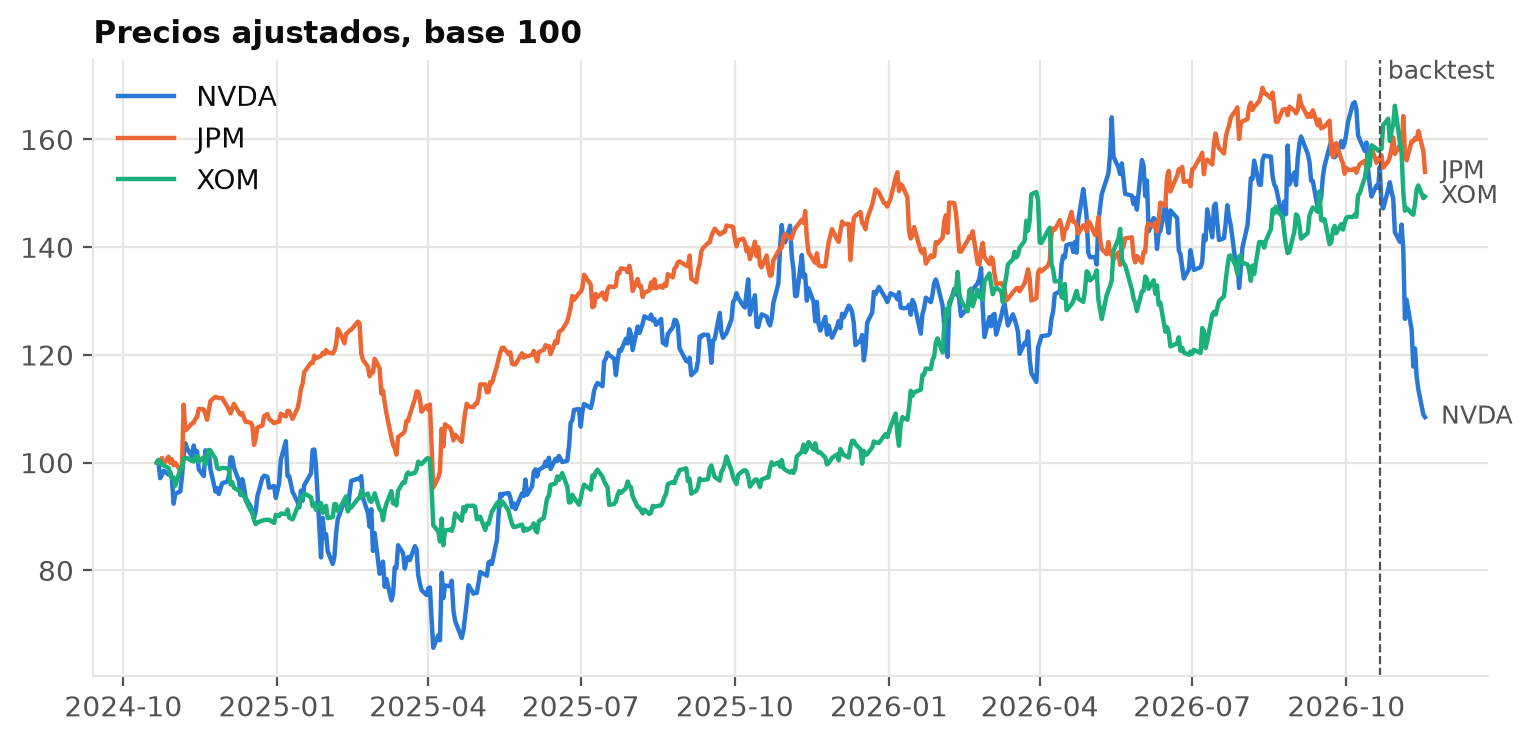
\includegraphics[width=0.8\textwidth]{01_precios.png}
\caption{Precios ajustados en base 100. La línea punteada marca el inicio de la ventana de backtest.}\label{fig:precios}
\end{figure}

\paragraph{Estadísticos descriptivos.}
La tabla~\ref{tab:desc} resume los rendimientos logarítmicos diarios de la ventana de entrenamiento. La dispersión es muy desigual: NVDA tiene casi el doble de volatilidad diaria que JPM y XOM. Los tres activos presentan curtosis en exceso positiva, es decir, colas más pesadas que las de una normal (cuya curtosis en exceso es cero); la de JPM (7.85) y la de NVDA (6.88) son especialmente altas. La prueba de Jarque--Bera rechaza la normalidad de los tres activos y del portafolio con $p<0.001$.

\begin{table}[H]
\centering
\renewcommand{\arraystretch}{1.2}
\begin{tabular}{@{}lrrrr@{}}
\toprule
 & \textbf{NVDA} & \textbf{JPM} & \textbf{XOM} & \textbf{Portafolio}\\
\midrule
Media diaria & 0.08\,\% & 0.09\,\% & 0.09\,\% & 0.11\,\%\\
Desviación diaria & 2.76\,\% & 1.55\,\% & 1.57\,\% & 1.33\,\%\\
Asimetría & $-0.32$ & 0.10 & $-0.51$ & 0.35\\
Curtosis en exceso & 6.88 & 7.85 & 1.78 & 11.41\\
Mínimo & $-18.6\,\%$ & $-7.8\,\%$ & $-7.5\,\%$ & ---\\
Máximo & 17.2\,\% & 10.9\,\% & 4.9\,\% & ---\\
Jarque--Bera & 995.3 & 1284.5 & 87.9 & 2722.5\\
\bottomrule
\end{tabular}
\caption{Estadísticos de los rendimientos logarítmicos diarios (entrenamiento). Para el portafolio, rendimiento simple según \eqref{eq:portafolio}. El valor crítico de Jarque--Bera al 5\,\% es 5.99.}\label{tab:desc}
\end{table}

La figura~\ref{fig:distribuciones} lo confirma de forma visual. Los histogramas son más picudos que la normal ajustada y los gráficos QQ se separan de la recta en los extremos: los eventos extremos son más frecuentes y de mayor magnitud que lo que supone la normal. El caso de XOM es más cercano a la normal en el centro, pero con una cola izquierda más larga.

\begin{figure}[H]
\centering
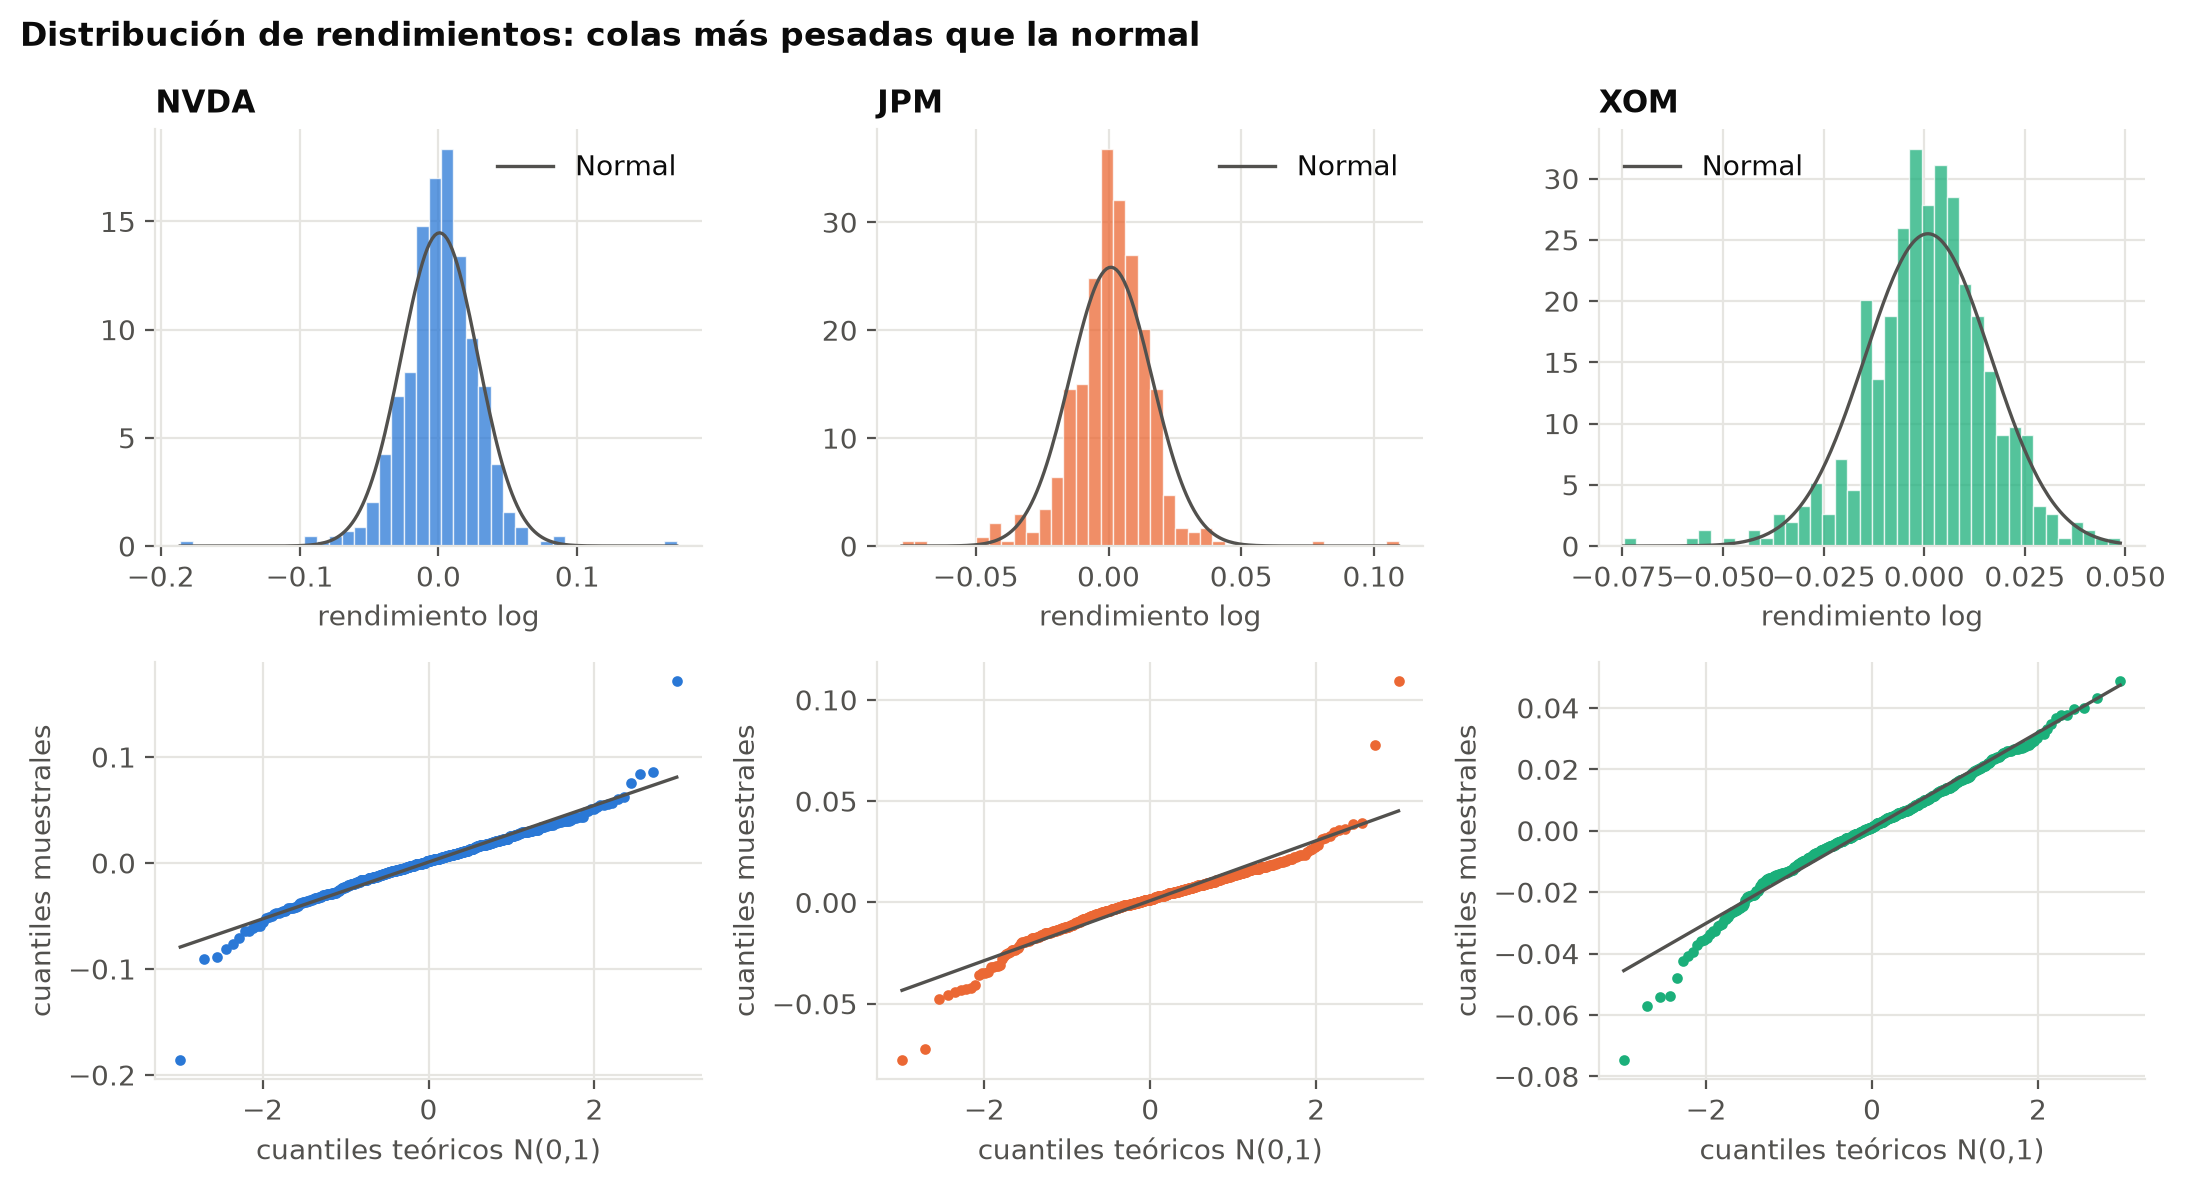
\includegraphics[width=0.92\textwidth]{01_distribuciones.png}
\caption{Distribución de los rendimientos logarítmicos de cada activo. Arriba, histograma con la normal ajustada; abajo, gráfico QQ frente a la normal.}\label{fig:distribuciones}
\end{figure}

\paragraph{Dependencia entre activos y portafolio.}
Las correlaciones son bajas (figura~\ref{fig:correlacion}): 0.32 entre NVDA y JPM, 0.15 entre JPM y XOM y prácticamente cero entre NVDA y XOM. Hay, por tanto, una diversificación real. El portafolio equiponderado tiene una desviación de $1.33\,\%$, menor que la de NVDA y similar a la de JPM y XOM, y una curtosis en exceso de 11.4, superior a la de cada activo por separado: la cola del portafolio sigue siendo pesada pese a la diversificación.

\begin{figure}[H]
\centering
\begin{minipage}{0.34\textwidth}
\centering
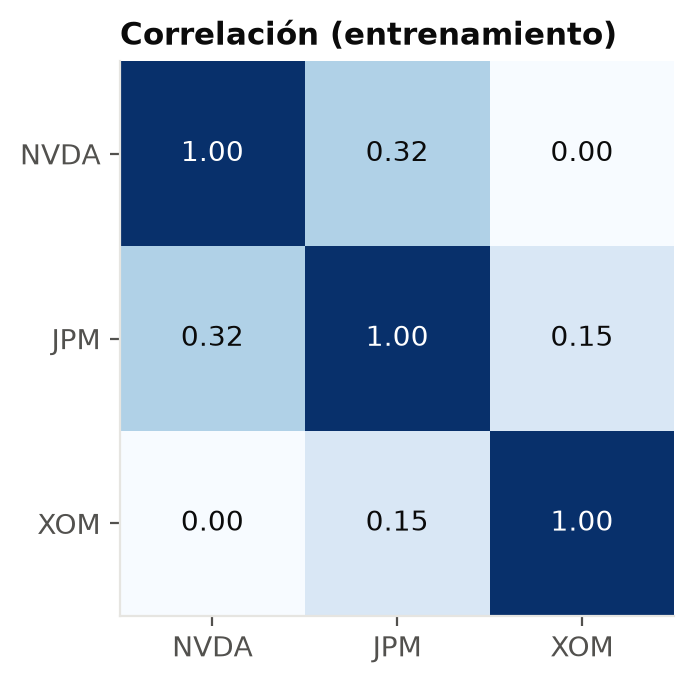
\includegraphics[width=\textwidth]{01_correlacion.png}
\caption{Correlación de los rendimientos (entrenamiento).}\label{fig:correlacion}
\end{minipage}\hfill
\begin{minipage}{0.60\textwidth}
\begin{cajaresultado}{Referencia histórica del portafolio}
Con los 500 días de entrenamiento, la simulación histórica da
\[
  \VaR_{95\%}=1.69\,\%,\qquad \ES_{95\%}=2.92\,\%.
\]
Estos valores son el punto de comparación para los dos modelos.
\end{cajaresultado}
\end{minipage}
\end{figure}

\begin{cajanota}{Implicación para el modelado}
La evidencia anticipa el resultado central del trabajo: como los datos tienen colas pesadas, un modelo normal debería \emph{subestimar} el riesgo en las colas lejanas (ES), aunque, como se verá, puede sobrestimar el VaR del 5\,\%. Una GAN, en cambio, podría en principio aprender la forma de la distribución, pero con solo 500 observaciones los eventos extremos son muy pocos para aprenderlos bien.
\end{cajanota}

% -------------------------------------------------------------------
\subsection{VaR al 95\,\% con Redes GAN (500 escenarios)}\label{sec:gan}

\paragraph{Arquitectura.}
Se implementó una GAN propia en PyTorch (anexo~B). El generador transforma un vector de ruido de dimensión 8 en un vector de rendimientos estandarizados de los 3 activos; el discriminador clasifica vectores de 3 rendimientos como reales o falsos. Ambos son perceptrones de dos capas ocultas de 64 neuronas con activación LeakyReLU (tabla~\ref{tab:gan}). El generador tiene 4\,931 parámetros y el discriminador 4\,481, un tamaño razonable para 500 observaciones de dimensión 3.

\begin{table}[H]
\centering
\renewcommand{\arraystretch}{1.2}
\begin{tabular}{@{}ll@{}}
\toprule
\textbf{Componente} & \textbf{Configuración}\\
\midrule
Generador $G$ & $8\to64\to64\to3$, LeakyReLU(0.2), sin activación a la salida\\
Discriminador $D$ & $3\to64\to64\to1$, LeakyReLU(0.2), dropout 0.2 en las capas ocultas\\
Pérdida & Entropía cruzada binaria; $G$ con pérdida no saturante \eqref{eq:LG}\\
Etiquetas reales & Suavizadas a 0.9 \eqref{eq:LD}\\
Optimizador & Adam, $\text{lr}=2\times10^{-4}$, $\beta_1=0.5$, $\beta_2=0.999$ (ambas redes)\\
Entrenamiento & 400 épocas, lote de 128, 4 lotes por época\\
EMA de pesos de $G$ & Factor 0.99 (se muestrea con $G_{\text{EMA}}$)\\
Entrada & Rendimientos log estandarizados con $\hat\mu,\hat\sigma$ de la ventana\\
Escenarios & 500 por día, $\hat{\mathbf r}=\hat{\bm\mu}+\hat{\bm\sigma}\odot G(\mathbf z)$\\
\bottomrule
\end{tabular}
\caption{Configuración de la GAN.}\label{tab:gan}
\end{table}

\paragraph{Procedimiento.}
Cada día de backtest $k=1,\dots,20$ usa los 500 rendimientos inmediatamente anteriores. Se entrena una GAN nueva, \emph{independiente} para cada día y con semilla propia, se generan 500 escenarios y se calcula el VaR a un día (algoritmo~\ref{alg:gan}). Es la forma de trabajar de un modelo que se recalibra periódicamente, y evita que el VaR de un día use información del día que se predice.

\begin{algorithm}[H]
\caption{VaR con GAN (para un día de backtest)}\label{alg:gan}
\Entrada{ventana $\{\mathbf r_s\}_{s=1}^{500}$, épocas $E=400$, lote $b=128$, escenarios $N=500$}
\Salida{$\widehat{\VaR}$ y $\widehat{\ES}$ a un día}
Estandarizar: $\mathbf x_s\leftarrow(\mathbf r_s-\hat{\bm\mu})/\hat{\bm\sigma}$\;
Inicializar $G$, $D$ y $G_{\text{EMA}}\leftarrow G$\;
\Para{época $=1,\dots,E$}{
  \Para{cada lote $\{\mathbf x_k\}_{k=1}^{b}$ de datos reales}{
    Muestrear $\mathbf z_k\sim\Normal(\mathbf 0,\mathbf I_8)$ y generar $G(\mathbf z_k)$\;
    Actualizar $D$ con un paso de Adam sobre $\mathcal L_D$ \eqref{eq:LD} \Comentario*[r]{reales$\to0.9$, falsas$\to0$}
    Actualizar $G$ con un paso de Adam sobre $\mathcal L_G$ \eqref{eq:LG} \Comentario*[r]{falsas$\to1$}
    $\theta_{\text{EMA}}\leftarrow0.99\,\theta_{\text{EMA}}+0.01\,\theta_G$\;
  }
}
Muestrear $\mathbf z^{(j)}\sim\Normal(\mathbf 0,\mathbf I_8)$ y obtener $\mathbf r^{(j)}=\hat{\bm\mu}+\hat{\bm\sigma}\odot G_{\text{EMA}}(\mathbf z^{(j)})$, $j=1,\dots,N$\;
$R^{(j)}\leftarrow\sum_i w_i\,(e^{r_i^{(j)}}-1)$; \quad $\widehat{\VaR},\widehat{\ES}\leftarrow$ cuantil y cola al $5\,\%$\;
\Retorna{$\widehat{\VaR},\widehat{\ES}$}
\end{algorithm}

\paragraph{Entrenamiento.}
La figura~\ref{fig:perdidas} muestra las pérdidas de ambas redes en la primera ventana. Ninguna colapsa a cero: terminan cerca de $1.38$ la de $D$ y de $0.75$ la de $G$. Son, de hecho, los valores de equilibrio cuando $D$ no puede distinguir entre real y falso: si $D$ responde una misma probabilidad $p$ para todas las muestras, su pérdida \eqref{eq:LD} se minimiza en $p=0.9/1.9\approx0.47$ y vale $\approx1.38$ (sin suavizado sería $2\ln2\approx1.39$), y la de $G$ \eqref{eq:LG} vale $-\ln p\approx0.75$. Las oscilaciones amplias de las primeras 250 épocas se amortiguan después, y las redes siguen compitiendo hasta el final. Es la señal de un entrenamiento sano, sin ganador absoluto, aunque, como se explicó, esto no garantiza por sí solo la calidad de las muestras.

\begin{figure}[H]
\centering
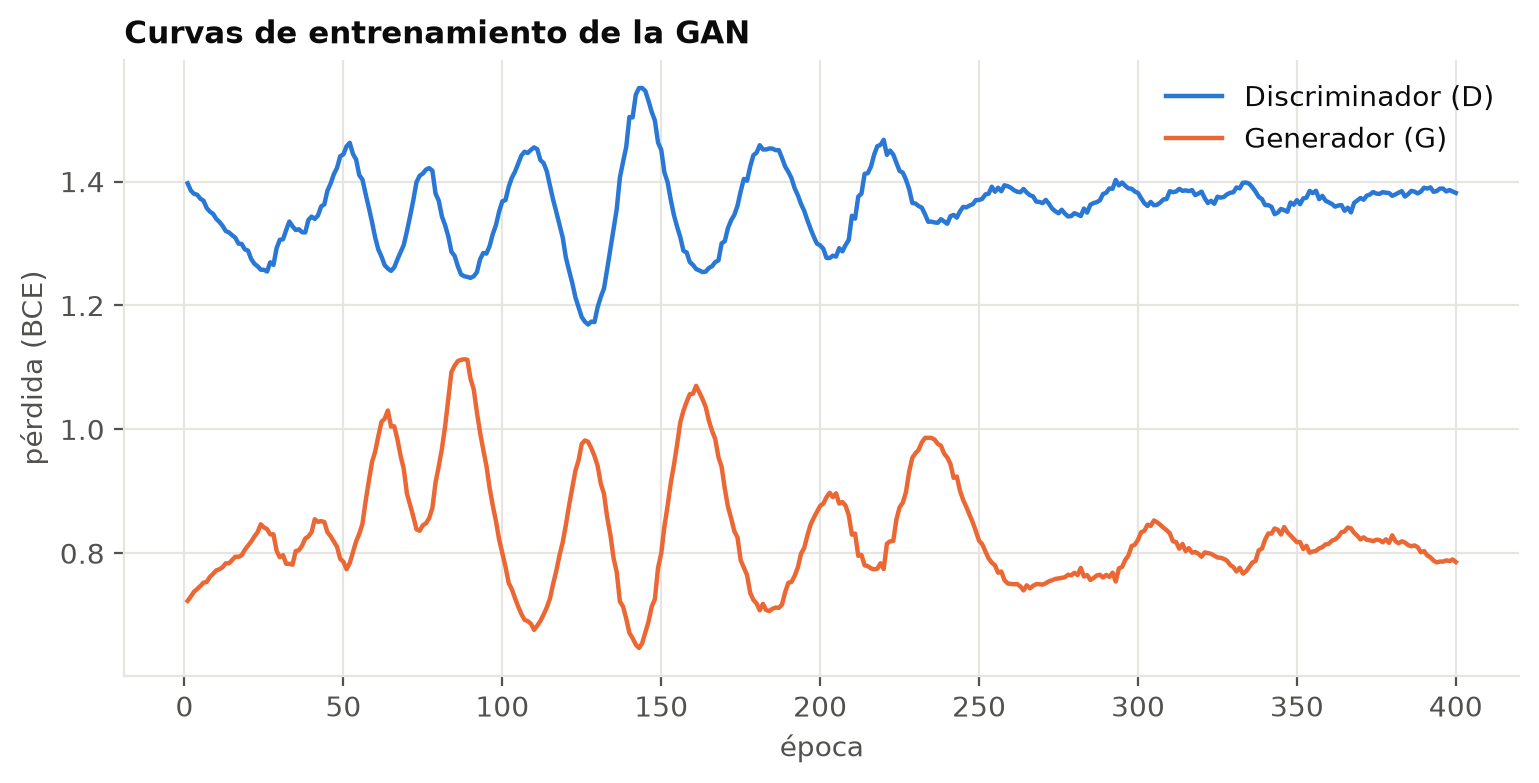
\includegraphics[width=0.72\textwidth]{02_gan_perdidas.png}
\caption{Pérdidas del discriminador y del generador durante las 400 épocas (primera ventana).}\label{fig:perdidas}
\end{figure}

\paragraph{Resultado en $t_0$.}
Para el primer día del backtest (21 de octubre de 2026), los 500 escenarios de la GAN dan un $\VaR_{95\%}=1.81\,\%$, con intervalo de confianza bootstrap del $95\,\%$ de $[1.62\,\%,\;2.00\,\%]$, y un $\ES_{95\%}=2.33\,\%$. El VaR de la GAN es el más cercano al histórico (1.69\,\%), que cae dentro de su intervalo. Pero el ES es menor que el histórico (2.92\,\%), lo que indica que la cola extrema está subestimada.

\paragraph{Qué aprende la GAN y qué no.}
Los escenarios de la GAN tienen desviación de $1.05\,\%$ frente a $1.33\,\%$ del historial, y curtosis en exceso de $0.25$ frente a $11.41$. La GAN aprende el \emph{cuerpo} de la distribución, pero no sus colas: los pocos eventos extremos de la ventana (como el $-18.6\,\%$ de NVDA) son probablemente demasiado raros para que el generador los aprenda. A esto se suma una distorsión de la dependencia, que se analiza en la sección~\ref{sec:mc}.

% -------------------------------------------------------------------
\subsection{VaR al 95\,\% vía Monte Carlo (500 escenarios)}\label{sec:mc}

\paragraph{Procedimiento.}
Se aplica el algoritmo~\ref{alg:mc} con la misma ventana móvil de 500 días, 500 escenarios por día y semilla $42+k$ (anexo~C). No requiere entrenamiento: basta estimar la media y la covarianza.

\paragraph{Comparación en $t_0$.}
La tabla~\ref{tab:t0} contrasta los dos modelos con el historial para el primer día de prueba, y la figura~\ref{fig:dist2} muestra las densidades y los gráficos QQ de los escenarios frente al historial.

\begin{table}[H]
\centering
\renewcommand{\arraystretch}{1.2}
\begin{tabular}{@{}lrrr@{}}
\toprule
 & \textbf{Historial (500 d)} & \textbf{GAN} & \textbf{Monte Carlo}\\
\midrule
Media diaria & 0.11\,\% & 0.13\,\% & 0.08\,\%\\
Desviación diaria & 1.33\,\% & 1.05\,\% & 1.41\,\%\\
Asimetría & 0.35 & $-0.53$ & 0.00\\
Curtosis en exceso & 11.41 & 0.25 & 0.12\\
\midrule
$\VaR_{95\%}$ & 1.69\,\% & 1.81\,\% & 2.19\,\%\\
IC 95\,\% bootstrap del VaR & --- & [1.62, 2.00]\,\% & [2.03, 2.41]\,\%\\
$\ES_{95\%}$ & 2.92\,\% & 2.33\,\% & 2.87\,\%\\
\bottomrule
\end{tabular}
\caption{Escenarios en $t_0$ (21-oct-2026): momentos del rendimiento del portafolio, VaR y ES.}\label{tab:t0}
\end{table}

\begin{figure}[H]
\centering
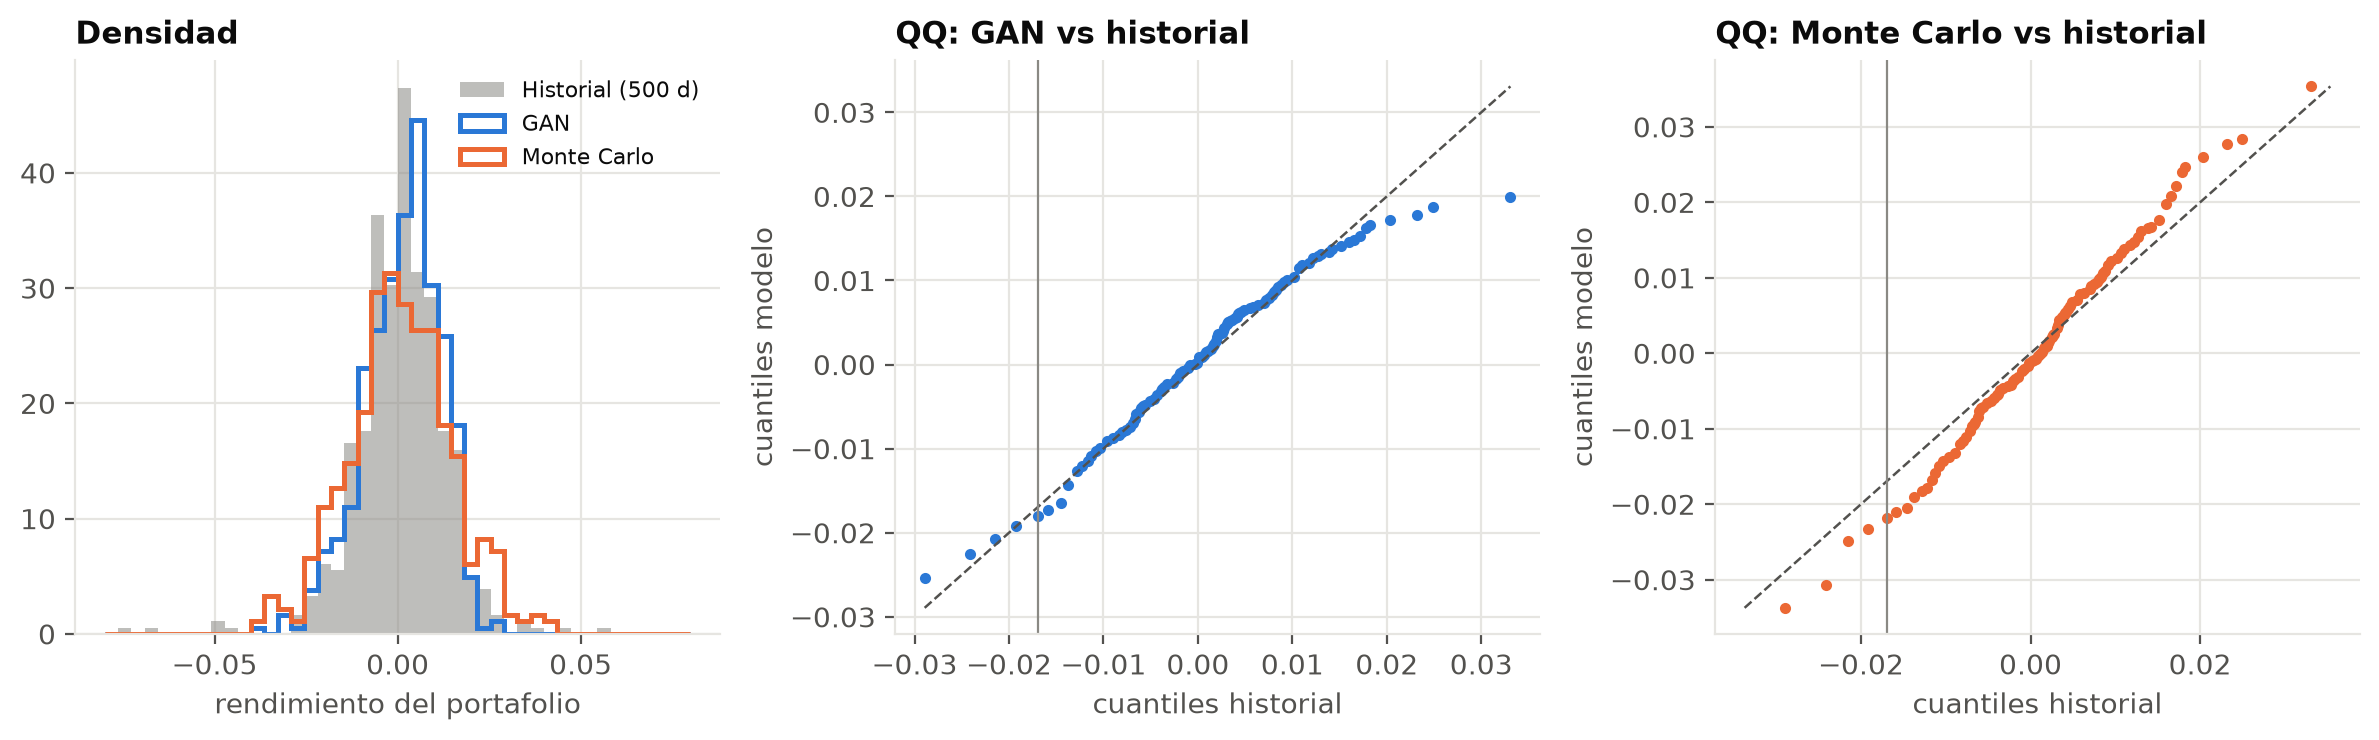
\includegraphics[width=0.94\textwidth]{02_distribuciones.png}
\caption{Rendimiento del portafolio en $t_0$. Izquierda: densidad del historial y de los escenarios de cada modelo. Centro y derecha: gráficos QQ de la GAN y de Monte Carlo frente al historial (la línea vertical marca el cuantil del $5\,\%$ histórico).}\label{fig:dist2}
\end{figure}

\paragraph{Lectura de los resultados.}
\begin{itemize}[nosep]
  \item Monte Carlo sobrestima el VaR (2.19\,\% frente a 1.69\,\%) \emph{y} reproduce bien el ES (2.87\,\% frente a 2.92\,\%). No es una contradicción. La distribución histórica es leptocúrtica: concentra mucha masa en el centro y una parte de su riesgo muy lejos, en la cola extrema. Una normal con la misma desviación reparte esa masa de forma más uniforme, así que pone más probabilidad en la región del cuantil del 5\,\% y su VaR resulta más alto. El ES, que promedia toda la cola, ya compensa ambos efectos. Dicho de otro modo, el VaR al 95\,\% se ve engañosamente conservador y el verdadero problema de la normal está en la cola lejana.
  \item La GAN subestima dispersión y colas. Su ES (2.33\,\%) queda por debajo del histórico, como su desviación y su curtosis (figura~\ref{fig:dist2}, centro: en ambas colas los cuantiles de la GAN son menos extremos que los del historial).
  \item Dependencia. La tabla~\ref{tab:corr} muestra que Monte Carlo reproduce razonablemente las correlaciones, porque usa directamente la matriz de covarianza, y la GAN las distorsiona: induce una correlación negativa entre NVDA y XOM ($-0.16$) donde en los datos es nula, y casi elimina la de JPM--XOM (0.00 frente a 0.15). Un generador de $\R^8\to\R^3$ sin una restricción explícita sobre la correlación no tiene por qué respetarla.
\end{itemize}

\begin{table}[H]
\centering
\renewcommand{\arraystretch}{1.2}
\begin{tabular}{@{}lrrr@{}}
\toprule
\textbf{Correlación} & \textbf{Historial} & \textbf{GAN} & \textbf{Monte Carlo}\\
\midrule
NVDA--JPM & 0.32 & 0.28 & 0.41\\
NVDA--XOM & 0.00 & $-0.16$ & 0.01\\
JPM--XOM & 0.15 & 0.00 & 0.18\\
\bottomrule
\end{tabular}
\caption{Correlaciones de los escenarios en $t_0$ frente a las del historial.}\label{tab:corr}
\end{table}

\paragraph{El VaR a lo largo de los 20 días.}
La figura~\ref{fig:var20} y la tabla~\ref{tab:var20} muestran los VaR de los 20 días de prueba. El de Monte Carlo es más estable (desviación $0.13$ puntos porcentuales, entre $1.85\,\%$ y $2.30\,\%$) y mayor que el de la GAN en 17 de los 20 días (las excepciones son el 5, el 16 y el 17 de noviembre). El de la GAN fluctúa más (desviación de $0.23$ p.p.; entre $1.45\,\%$ y $2.36\,\%$), en parte porque se \emph{re-entrena de forma independiente} cada día con otra semilla, así que a la variación de los datos se suma la de la optimización.

\begin{figure}[H]
\centering
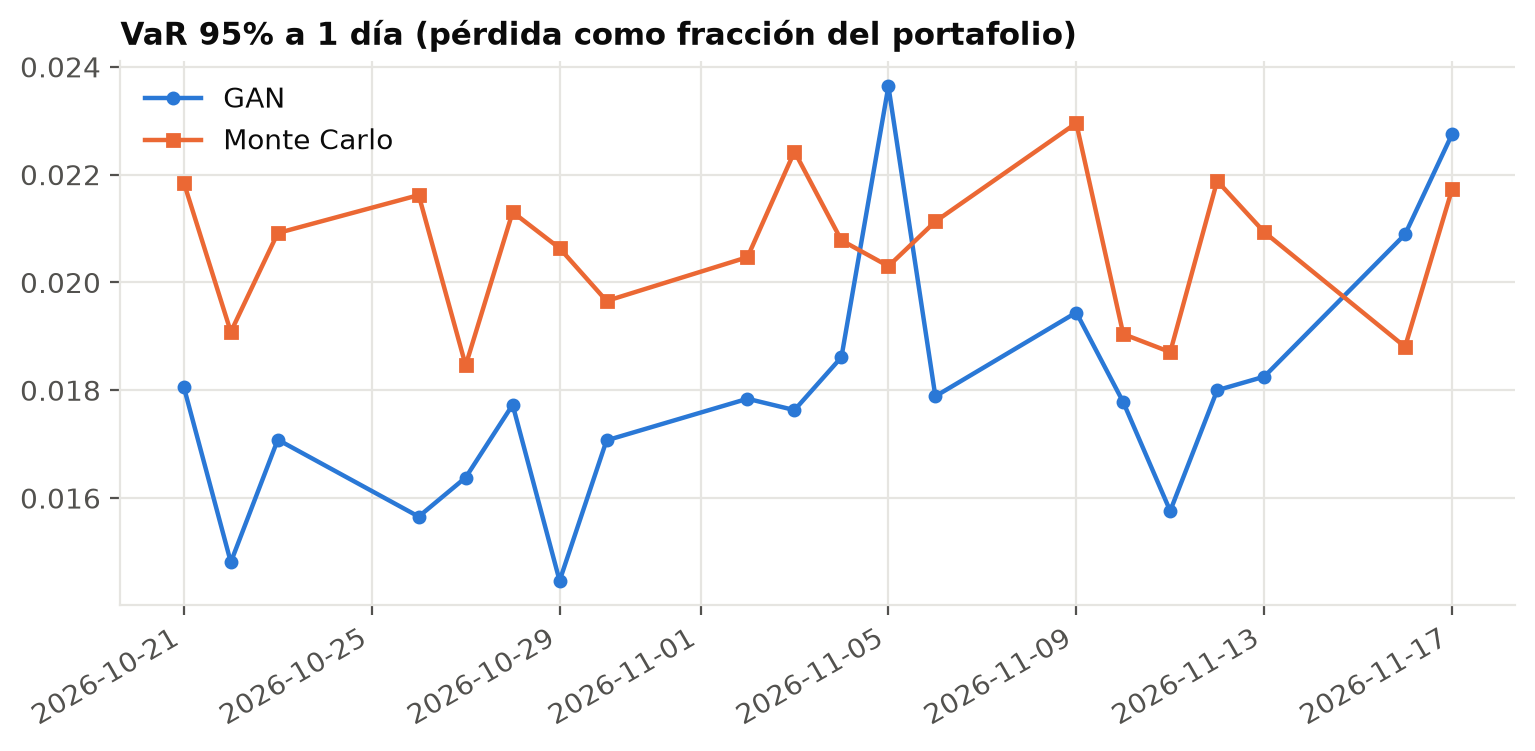
\includegraphics[width=0.72\textwidth]{02_var_20dias.png}
\caption{VaR al 95\,\% a un día de cada modelo durante los 20 días de prueba.}\label{fig:var20}
\end{figure}

\begin{table}[H]
\centering
\renewcommand{\arraystretch}{1.2}
\begin{tabular}{@{}llrrrr@{}}
\toprule
\textbf{Modelo} & \textbf{Medida} & \textbf{Media} & \textbf{Desv.} & \textbf{Mín.} & \textbf{Máx.} \\
\midrule
GAN propia & VaR 95\,\% & 1.80\,\% & 0.23\,\% & 1.45\,\% & 2.36\,\% \\
GAN propia & ES 95\,\% & 2.28\,\% & 0.24\,\% & 2.02\,\% & 2.98\,\% \\
Monte Carlo & VaR 95\,\% & 2.06\,\% & 0.13\,\% & 1.85\,\% & 2.30\,\% \\
Monte Carlo & ES 95\,\% & 2.59\,\% & 0.19\,\% & 2.24\,\% & 2.92\,\% \\
\bottomrule
\end{tabular}

\caption{VaR y ES a un día a lo largo de los 20 días del backtest.}\label{tab:var20}
\end{table}

% -------------------------------------------------------------------
\subsection{Backtest para 20 días}\label{sec:backtest}

Para cada día $t$ de prueba, el VaR se calcula con los 500 días anteriores y se compara con el rendimiento del portafolio que se observó ese día (sección~\ref{sec:teoria-backtest}). La tabla~\ref{tab:diaria} lista el detalle y la figura~\ref{fig:backtest} lo muestra: las barras son los rendimientos reales y la línea es $-\VaR$; una excepción ocurre cuando la barra baja más que la línea.

\begin{figure}[H]
\centering
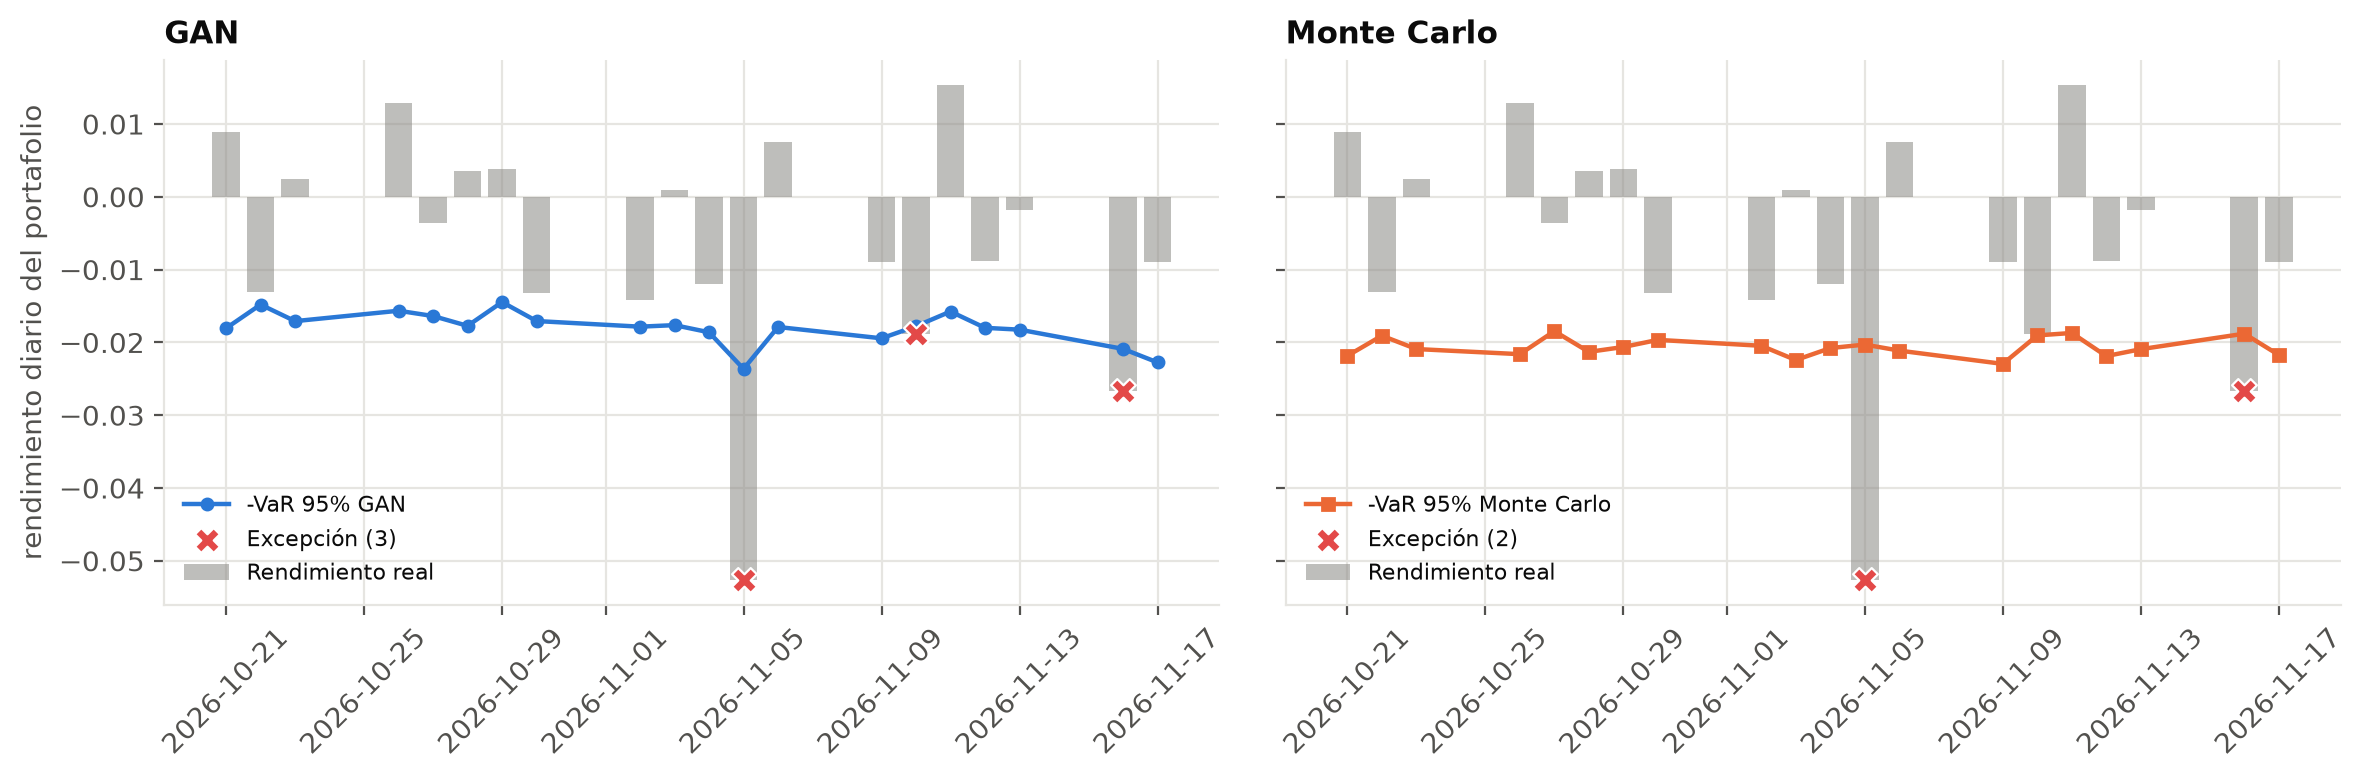
\includegraphics[width=0.94\textwidth]{03_backtest.png}
\caption{Backtest de 20 días. Barras: rendimiento real del portafolio. Línea: $-\VaR_{95\%}$. Las cruces son las excepciones.}\label{fig:backtest}
\end{figure}

\begin{table}[H]
\centering
\small
\renewcommand{\arraystretch}{1.1}
\begin{tabular}{@{}rlrrcrc@{}}
\toprule
 & & & \multicolumn{2}{c}{\textbf{GAN propia}} & \multicolumn{2}{c}{\textbf{Monte Carlo}} \\
\cmidrule(lr){4-5}\cmidrule(lr){6-7}
\textbf{Día} & \textbf{Fecha} & \textbf{Rend. real} & \textbf{VaR 95\,\%} & \textbf{Exc.} & \textbf{VaR 95\,\%} & \textbf{Exc.} \\
\midrule
1 & 21-oct & +0.88\,\% & 1.81\,\% & -- & 2.19\,\% & -- \\
2 & 22-oct & $-$1.31\,\% & 1.48\,\% & -- & 1.91\,\% & -- \\
3 & 23-oct & +0.24\,\% & 1.71\,\% & -- & 2.09\,\% & -- \\
4 & 26-oct & +1.29\,\% & 1.57\,\% & -- & 2.16\,\% & -- \\
5 & 27-oct & $-$0.36\,\% & 1.64\,\% & -- & 1.85\,\% & -- \\
6 & 28-oct & +0.35\,\% & 1.77\,\% & -- & 2.13\,\% & -- \\
7 & 29-oct & +0.39\,\% & 1.45\,\% & -- & 2.06\,\% & -- \\
8 & 30-oct & $-$1.32\,\% & 1.71\,\% & -- & 1.97\,\% & -- \\
9 & 2-nov & $-$1.42\,\% & 1.78\,\% & -- & 2.05\,\% & -- \\
10 & 3-nov & +0.10\,\% & 1.76\,\% & -- & 2.24\,\% & -- \\
11 & 4-nov & $-$1.20\,\% & 1.86\,\% & -- & 2.08\,\% & -- \\
12 & 5-nov & $-$5.27\,\% & \textbf{2.36\,\%} & \textbf{Sí} & \textbf{2.03\,\%} & \textbf{Sí} \\
13 & 6-nov & +0.76\,\% & 1.79\,\% & -- & 2.11\,\% & -- \\
14 & 9-nov & $-$0.90\,\% & 1.94\,\% & -- & 2.30\,\% & -- \\
15 & 10-nov & $-$1.88\,\% & \textbf{1.78\,\%} & \textbf{Sí} & 1.90\,\% & -- \\
16 & 11-nov & +1.54\,\% & 1.58\,\% & -- & 1.87\,\% & -- \\
17 & 12-nov & $-$0.89\,\% & 1.80\,\% & -- & 2.19\,\% & -- \\
18 & 13-nov & $-$0.18\,\% & 1.83\,\% & -- & 2.09\,\% & -- \\
19 & 16-nov & $-$2.66\,\% & \textbf{2.09\,\%} & \textbf{Sí} & \textbf{1.88\,\%} & \textbf{Sí} \\
20 & 17-nov & $-$0.89\,\% & 2.27\,\% & -- & 2.17\,\% & -- \\
\bottomrule
\end{tabular}

\caption{Backtest día por día. Las celdas en negrita son excepciones (la pérdida real supera el VaR).}\label{tab:diaria}
\end{table}

\paragraph{Resultados.}
La tabla~\ref{tab:bt} resume el backtest. La GAN tiene 3 excepciones (15\,\%) y Monte Carlo 2 (10\,\%), contra 1 esperada en cada caso.

\begin{table}[H]
\centering
\renewcommand{\arraystretch}{1.2}
\begin{tabular}{@{}lrr@{}}
\toprule
 & \textbf{GAN propia} & \textbf{Monte Carlo}\\
\midrule
Excepciones (esperadas: 1) & 3 & 2\\
Tasa de excepciones & 15\,\% & 10\,\%\\
Estadístico $LR_{uc}$ de Kupiec & 2.81 & 0.83\\
$p$-valor de Kupiec & 0.094 & 0.363\\
Exceso medio sobre el VaR (en excepciones) & 1.19 p.p. & 2.01 p.p.\\
VaR medio & 1.80\,\% & 2.06\,\%\\
Pérdida cuantílica media & 0.00237 & 0.00272\\
\bottomrule
\end{tabular}
\caption{Resumen del backtest a 20 días.}\label{tab:bt}
\end{table}

\paragraph{Las excepciones.}
Ocurrieron en tres fechas (tabla~\ref{tab:exc}). Ambos modelos fallan el 5 y el 16 de noviembre; la GAN falla, además, el 10 de noviembre, por un margen mínimo ($-1.88\,\%$ frente a un VaR de $1.78\,\%$). El 5 de noviembre es el día determinante: el portafolio cayó $5.27\,\%$ porque \emph{los tres activos} cayeron a la vez (NVDA $-9.3\,\%$, JPM $-4.2\,\%$, XOM $-2.4\,\%$), pese a que su correlación histórica es baja. Ese tipo de movimiento conjunto es el que un modelo con correlaciones estimadas en épocas normales no anticipa.

\begin{table}[H]
\centering
\renewcommand{\arraystretch}{1.2}
\begin{tabular}{@{}lrrr@{}}
\toprule
\textbf{Fecha} & \textbf{Rendimiento real} & \textbf{VaR GAN} & \textbf{VaR Monte Carlo}\\
\midrule
5-nov-2026 & $-5.27\,\%$ & 2.36\,\% (falla) & 2.03\,\% (falla)\\
10-nov-2026 & $-1.88\,\%$ & 1.78\,\% (falla) & 1.90\,\% (no falla)\\
16-nov-2026 & $-2.66\,\%$ & 2.09\,\% (falla) & 1.88\,\% (falla)\\
\bottomrule
\end{tabular}
\caption{Días con excepción.}\label{tab:exc}
\end{table}

\paragraph{Interpretación estadística.}
La prueba de Kupiec \emph{no rechaza} a ninguno de los dos modelos al $5\,\%$ ($p=0.094$ para la GAN y $p=0.363$ para Monte Carlo). Esto es lo que se esperaba dada la baja potencia de la prueba: con 20 días se necesitan al menos 4 excepciones para rechazar. Más aún, incluso si el modelo fuera perfecto, observar 2 o más excepciones ocurre con probabilidad del $26.4\,\%$ y 3 o más con $7.5\,\%$. Las 3 excepciones de la GAN son, entonces, un indicio de posible subestimación del riesgo, pero no una prueba. Por último, el resultado depende de un solo día: el $-5.27\,\%$ supera con holgura el VaR de ambos modelos.

% -------------------------------------------------------------------
\subsection{Comparación de los modelos y elección del finalista}\label{sec:comparacion}

\paragraph{Ranking.}
Con los cuatro criterios definidos en el marco teórico se obtiene la tabla~\ref{tab:ranking}. Cada modelo gana en dos criterios y la suma de rangos es 6 para ambos: \emph{el ranking empata}. Monte Carlo gana en calibración de la cobertura (2 excepciones frente a 3) y en distancia KS (0.076 frente a 0.090); la GAN gana en pérdida cuantílica (0.00237 frente a 0.00272) y en VaR medio (1.80\,\% frente a 2.06\,\%).

\begin{table}[H]
\centering
\renewcommand{\arraystretch}{1.2}
\begin{tabular}{@{}lrrrrl@{}}
\toprule
 & \multicolumn{2}{c}{\textbf{Valor}} & \multicolumn{2}{c}{\textbf{Rango}} & \\
\cmidrule(lr){2-3}\cmidrule(lr){4-5}
\textbf{Criterio} & \textbf{GAN} & \textbf{MC} & \textbf{GAN} & \textbf{MC} & \textbf{Mejor}\\
\midrule
Desviación de excepciones $|x-n\alpha|$ & 2 & 1 & 2 & 1 & MC\\
Pérdida cuantílica media & 0.00237 & 0.00272 & 1 & 2 & GAN\\
VaR medio & 1.80\,\% & 2.06\,\% & 1 & 2 & GAN\\
Distancia KS frente al historial & 0.090 & 0.076 & 2 & 1 & MC\\
\midrule
\textbf{Suma de rangos} & & & \textbf{6} & \textbf{6} & empate\\
\bottomrule
\end{tabular}
\caption{Ranking de los modelos (1 = mejor).}\label{tab:ranking}
\end{table}

\begin{cajaresultado}{Finalista según la regla declarada: GAN propia}
Como el ranking empata, se aplica el desempate fijado de antemano: la menor pérdida cuantílica. Gana la GAN propia ($0.00237$ frente a $0.00272$). Es una victoria por desempate, no por una ventaja amplia, y la siguiente subsección explica por qué hay que leerla con cautela.
\end{cajaresultado}

\paragraph{Por qué la elección es frágil.}
\begin{enumerate}[label=\arabic*., nosep]
  \item La pérdida cuantílica depende de un solo día. La diferencia entre modelos (0.00237 frente a 0.00272) está dominada por el 5 de noviembre.
  \item Un VaR menor solo es una ventaja si la cobertura es adecuada. El VaR medio de la GAN es más bajo, pero también lo es su cobertura: tiene más excepciones, aunque Kupiec no las rechace.
  \item La GAN depende de la semilla de entrenamiento. Se entrenó la GAN 8 veces con la misma ventana y los mismos 500 escenarios, cambiando solo la semilla (figura~\ref{fig:semillas}). El VaR en $t_0$ tuvo media $1.79\,\%$, desviación $0.17$ p.p. y rango $[1.58\,\%,\;2.11\,\%]$. Ese rango es comparable a la distancia entre ambos modelos ($1.81\,\%$ y $2.19\,\%$ en $t_0$): con otra semilla la GAN habría quedado mucho más cerca de Monte Carlo o del historial.
  \item El error de muestreo es del mismo orden. Con solo 500 escenarios, los intervalos bootstrap del VaR miden unos $\pm0.2$ p.p. (figura~\ref{fig:ic}), de acuerdo con la ecuación \eqref{eq:varcuantil}. Cada intervalo mide unos $0.4$ p.p. de ancho, comparable a la diferencia entre los dos VaR ($0.38$ p.p.). En $t_0$ los intervalos de la GAN ($[1.62,\,2.00]$) y de Monte Carlo ($[2.03,\,2.41]$) no se traslapan, de modo que el error de muestreo por sí solo no explicaría la diferencia; pero la variabilidad por semilla del punto anterior sí la cubre.
\end{enumerate}

\begin{figure}[H]
\centering
\begin{subfigure}{0.58\textwidth}
\centering
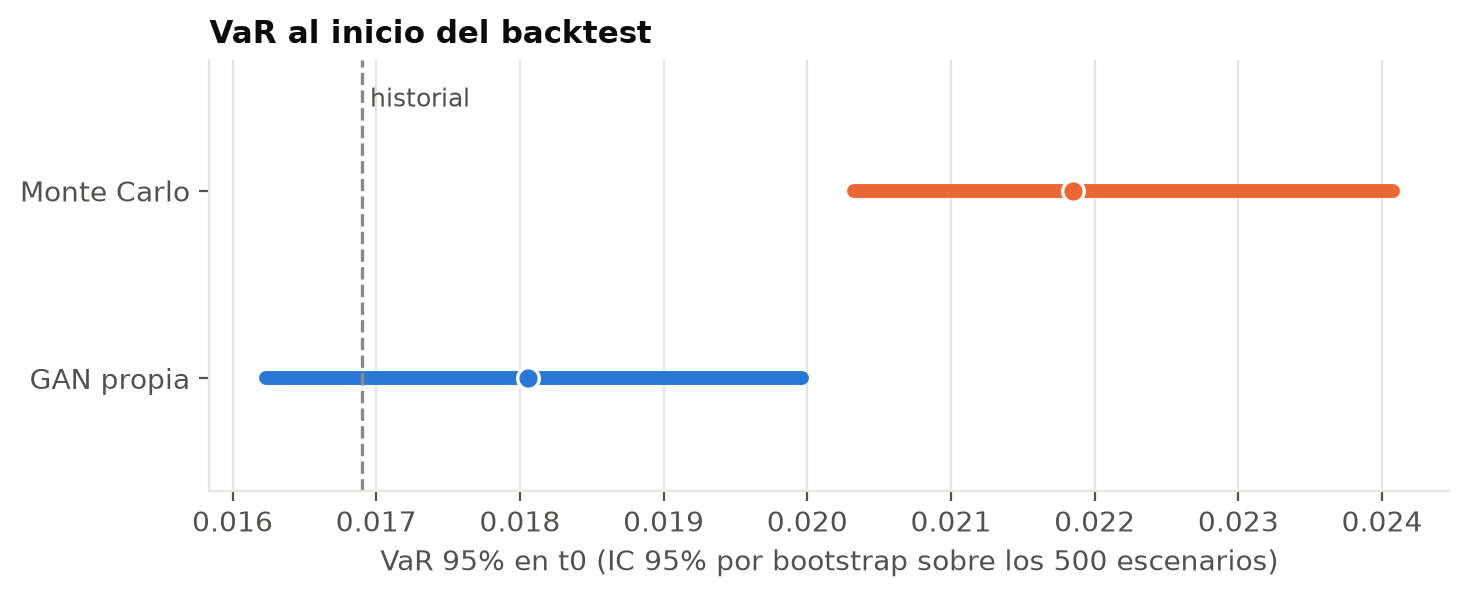
\includegraphics[width=\textwidth]{04_ic_var.png}
\caption{IC bootstrap del VaR en $t_0$.}\label{fig:ic}
\end{subfigure}\hfill
\begin{subfigure}{0.40\textwidth}
\centering
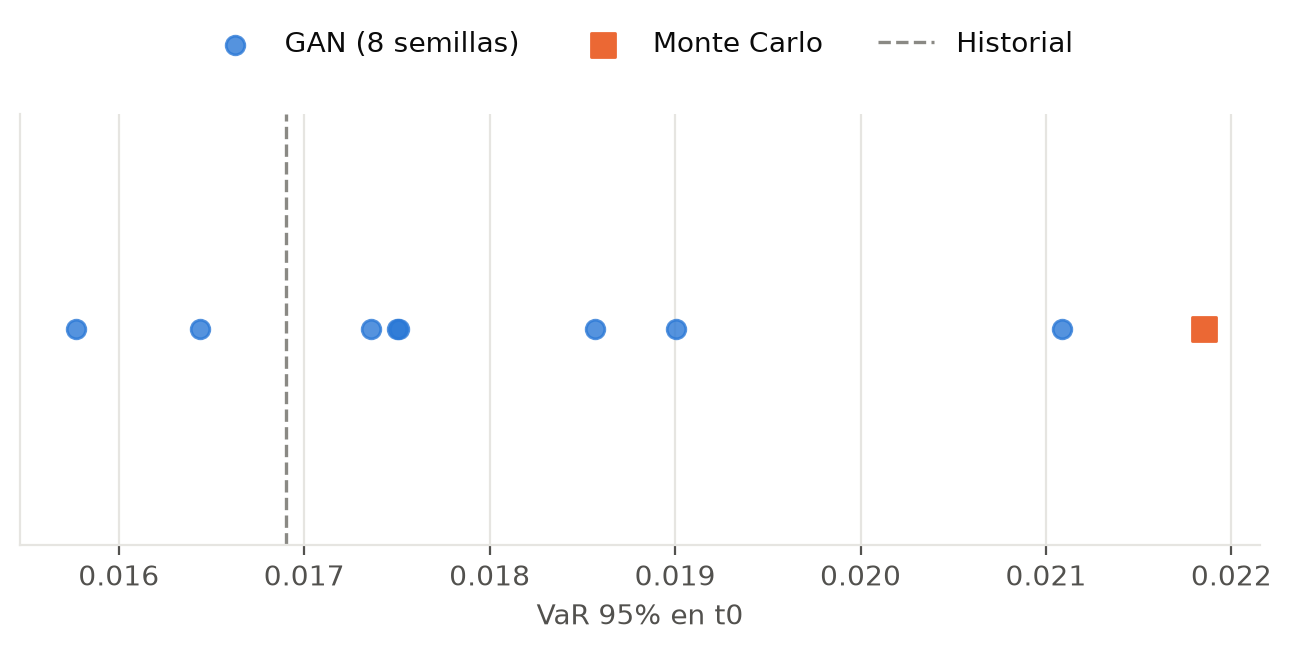
\includegraphics[width=\textwidth]{04_robustez_semillas.png}
\caption{VaR de la GAN con 8 semillas.}\label{fig:semillas}
\end{subfigure}
\caption{Incertidumbre del VaR en $t_0$. Línea punteada: VaR histórico (1.69\,\%).}\label{fig:incertidumbre}
\end{figure}

\paragraph{Lectura conjunta.}
La tabla~\ref{tab:cualitativa} reúne la evidencia más allá del ranking. Si el criterio prioritario fuera acertar el VaR del 5\,\% con la menor holgura posible, la GAN es el modelo competitivo. Si fuera la fiabilidad del ES, la estabilidad y la dependencia entre activos, el modelo prudente sería Monte Carlo.

\begin{table}[H]
\centering
\small
\renewcommand{\arraystretch}{1.25}
\begin{tabular}{@{}p{4.6cm}p{5.1cm}p{5.1cm}@{}}
\toprule
\textbf{Aspecto} & \textbf{GAN propia} & \textbf{Monte Carlo}\\
\midrule
VaR 95\,\% en $t_0$ frente al histórico (1.69\,\%) & 1.81\,\% (IC contiene al histórico) & 2.19\,\% (IC no lo contiene)\\
ES 95\,\% en $t_0$ frente al histórico (2.92\,\%) & 2.33\,\% (subestima) & 2.87\,\% (casi igual)\\
Dependencia entre activos & Distorsionada & Fiel (usa $\hat{\bm\Sigma}$)\\
Estabilidad del VaR (desviación en 20 días) & 0.23 p.p. & 0.13 p.p.\\
Sensibilidad a la semilla & Alta (rango 1.58--2.11\,\%) & Solo ruido de muestreo\\
Excepciones (esperada: 1) & 3 & 2\\
Pérdida cuantílica & Menor & Mayor\\
Costo computacional & Entrenar 20 redes & Inmediato\\
\bottomrule
\end{tabular}
\caption{Resumen cualitativo de la comparación.}\label{tab:cualitativa}
\end{table}

\begin{cajanota}{Decisión}
Finalista: GAN propia, siguiendo la regla fijada de antemano. Con la salvedad, que el trabajo documenta, de que los datos \emph{no permiten afirmar que un modelo sea mejor que el otro}: el empate en el ranking, el backtest de solo 20 días, el efecto de un único día extremo y la variabilidad por semilla son del mismo orden que la diferencia entre ambos.
\end{cajanota}

% ===================================================================
%  4. CONCLUSIONES
% ===================================================================
\section{Conclusiones del trabajo}\label{sec:conclusiones}

\begin{enumerate}[label=\arabic*., itemsep=2mm]
  \item Los datos justifican explorar alternativas a la normal. Los rendimientos de NVDA, JPM y XOM tienen colas pesadas (curtosis en exceso de 1.8 a 7.8 por activo y de 11.4 para el portafolio) y la prueba de Jarque--Bera rechaza la normalidad con claridad.
  \item La GAN es competitiva en VaR. En $t_0$ estima $1.81\,\%$ frente a $1.69\,\%$ del historial, con un intervalo que contiene al valor histórico, y obtiene la menor pérdida cuantílica del backtest. Con ello resulta la finalista según la regla declarada.
  \item Pero falla donde más importa para el riesgo de cola. Su ES (2.33\,\%) y su curtosis (0.25) quedan muy por debajo de los históricos, las correlaciones entre activos salen distorsionadas y el VaR cambia entre $1.58\,\%$ y $2.11\,\%$ solo por cambiar la semilla. La GAN aprende el cuerpo de la distribución, no sus colas.
  \item Monte Carlo es más estable y más fiel en el ES. Sobrestima el VaR del 5\,\% (2.19\,\%), pero su ES (2.87\,\%) casi coincide con el histórico y reproduce la dependencia entre activos. Es el modelo prudente si la prioridad es la fiabilidad del ES o la estabilidad.
  \item Con 20 días de backtest no hay evidencia para declarar un ganador. Kupiec no rechaza a ningún modelo (se necesitarían al menos 4 excepciones), el ranking empata 6 a 6 y todo depende del día del $-5.27\,\%$, en que los tres activos cayeron a la vez.
\end{enumerate}

\subsection*{Limitaciones}

\begin{itemize}[nosep]
  \item Backtest corto (20 días), que además cae en un régimen de volatilidad mayor que el de entrenamiento.
  \item Una sola GAN por día, con una sola semilla; la variabilidad entre semillas es comparable a la diferencia entre modelos.
  \item La GAN modela vectores diarios independientes: no captura aglomeración de volatilidad ni dependencia temporal.
  \item El único modelo de referencia es la normal multivariada; no se incluyó uno con colas pesadas.
  \item Portafolio de solo tres acciones, con pesos fijos y horizonte de un día.
\end{itemize}

\subsection*{Trabajo futuro}

\begin{itemize}[nosep]
  \item Ampliar el backtest (por ejemplo, 250 días) y entrenar varias semillas por día para promediar el ruido de entrenamiento.
  \item Usar arquitecturas que modelen ventanas y volatilidad condicional, como TimeGAN o GAN con convoluciones temporales \cite{takahashi2019, yoon2019}.
  \item Agregar referencias con colas pesadas: simulación histórica y $t$ de Student multivariada.
  \item Incorporar pruebas de independencia de las excepciones (por ejemplo, Christoffersen) cuando haya más días.
\end{itemize}

% ===================================================================
%  ANEXOS
% ===================================================================
\clearpage
\section*{Anexos}
\addcontentsline{toc}{section}{Anexos}

\subsection*{Anexo A. Estructura del repositorio y ejecución}
\addcontentsline{toc}{subsection}{Anexo A. Estructura del repositorio y ejecución}

El código se organiza siguiendo la estructura del proyecto: un script por cada paso, módulos compartidos y un cuaderno de análisis por sección.

El repositorio del proyecto está disponible en GitHub: \url{https://github.com/CFabianEsteva/VaR-con-redes-GAN}.

\begin{lstlisting}[language={}, numbers=none, basicstyle=\ttfamily\footnotesize]
.
|-- data/                    precios.csv, rendimientos.csv
|-- src/
|   |-- config.py            parametros globales (activos, ventanas, GAN)
|   |-- utils.py             datos, portafolio, VaR/ES, Kupiec, perdida cuantilica
|   |-- gan.py               GAN propia (PyTorch)
|   |-- montecarlo.py        simulacion Monte Carlo (normal multivariada)
|   |-- 01_descarga_datos.py     3.1  descarga de precios y rendimientos
|   |-- 02_var_redes_gan.py      3.2  VaR con la GAN
|   |-- 03_var_montecarlo.py     3.3  VaR via Monte Carlo
|   |-- 04_backtest.py           3.4  backtest a 20 dias
|   `-- 05_evaluacion.py         3.5  comparacion y finalista
|-- notebooks/               01_eda, 02_var, 03_backtest, 04_evaluation
|-- results/                 CSV con VaR, backtest y finalista
`-- figures/                 graficas de los notebooks
\end{lstlisting}

Para reproducir los resultados:

\begin{lstlisting}[language=bash, numbers=none, basicstyle=\ttfamily\footnotesize]
pip install -r requirements.txt
cd src
python 01_descarga_datos.py   # descarga y rendimientos
python 02_var_redes_gan.py    # VaR con GAN (entrena una GAN por dia)
python 03_var_montecarlo.py   # VaR con Monte Carlo
python 04_backtest.py         # excepciones, Kupiec, perdida cuantilica
python 05_evaluacion.py       # ranking y finalista
\end{lstlisting}

Las semillas son fijas (\texttt{SEED = 42}, y \texttt{SEED + k} para el día $k$), de modo que los escenarios son reproducibles en un mismo entorno. Los datos de precios son los de \texttt{data/precios.csv}.

\anexo{Anexo B. Código de la GAN (\texttt{gan.py})}
\lstinputlisting[basicstyle=\ttfamily\scriptsize]{codigo/gan.py}

\anexo{Anexo C. Monte Carlo y funciones de riesgo (\texttt{montecarlo.py}, \texttt{utils.py})}
\lstinputlisting[basicstyle=\ttfamily\scriptsize]{codigo/montecarlo.py}
\vspace{4mm}
\lstinputlisting[basicstyle=\ttfamily\scriptsize, firstline=25]{codigo/utils.py}


% ===================================================================
%  BIBLIOGRAFÍA
% ===================================================================
\bigskip
\addcontentsline{toc}{section}{Bibliografía}
\begin{thebibliography}{99}
\setlength{\itemsep}{2pt}
\footnotesize

\bibitem{googlegan} Google for Developers. \emph{Generative Adversarial Networks}. Curso de Machine Learning. \url{https://developers.google.com/machine-learning/gan}. Consultado en noviembre de 2026.

\bibitem{takahashi2019} Takahashi, S., Chen, Y., \& Tanaka-Ishii, K. (2019). Modeling financial time-series with generative adversarial networks. \emph{Physica A: Statistical Mechanics and its Applications}, 527, 121261. \url{https://doi.org/10.1016/j.physa.2019.121261}

\bibitem{yoon2019} Yoon, J., Jarrett, D., \& van der Schaar, M. (2019). Time-series generative adversarial networks. En \emph{Advances in Neural Information Processing Systems}, 32. Curran Associates, Inc. \url{https://proceedings.neurips.cc/paper_files/paper/2019/file/c9efe5f26cd17ba6216bbe2a7d26d490-Paper.pdf}

\bibitem{goodfellow2014} Goodfellow, I. J., Pouget-Abadie, J., Mirza, M., Xu, B., Warde-Farley, D., Ozair, S., Courville, A., \& Bengio, Y. (2014). Generative adversarial nets. En \emph{Advances in Neural Information Processing Systems}, 27. Curran Associates, Inc. \url{https://proceedings.neurips.cc/paper_files/paper/2014/file/f033ed80deb0234979a61f95710dbe25-Paper.pdf}

\bibitem{jorion2007} Jorion, P. (2007). \emph{Value at Risk: The New Benchmark for Managing Financial Risk} (3.ª ed.). McGraw-Hill.

\bibitem{acerbi2002} Acerbi, C., \& Tasche, D. (2002). On the coherence of expected shortfall. \emph{Journal of Banking \& Finance}, 26(7), 1487--1503.

\bibitem{glasserman2004} Glasserman, P. (2004). \emph{Monte Carlo Methods in Financial Engineering}. Springer.

\bibitem{cont2001} Cont, R. (2001). Empirical properties of asset returns: stylized facts and statistical issues. \emph{Quantitative Finance}, 1(2), 223--236.

\bibitem{kupiec1995} Kupiec, P. H. (1995). Techniques for verifying the accuracy of risk measurement models. \emph{The Journal of Derivatives}, 3(2), 73--84.

\bibitem{koenker1978} Koenker, R., \& Bassett, G. (1978). Regression quantiles. \emph{Econometrica}, 46(1), 33--50.

\bibitem{kingma2015} Kingma, D. P., \& Ba, J. (2015). Adam: A method for stochastic optimization. En \emph{International Conference on Learning Representations (ICLR)}.

\bibitem{salimans2016} Salimans, T., Goodfellow, I., Zaremba, W., Cheung, V., Radford, A., \& Chen, X. (2016). Improved techniques for training GANs. En \emph{Advances in Neural Information Processing Systems}, 29.

\bibitem{srivastava2014} Srivastava, N., Hinton, G., Krizhevsky, A., Sutskever, I., \& Salakhutdinov, R. (2014). Dropout: a simple way to prevent neural networks from overfitting. \emph{Journal of Machine Learning Research}, 15(56), 1929--1958.

\bibitem{yazici2019} Yazıcı, Y., Foo, C.-S., Winkler, S., Yap, K.-H., Piliouras, G., \& Chandrasekhar, V. (2019). The unusual effectiveness of averaging in GAN training. En \emph{International Conference on Learning Representations (ICLR)}.

\end{thebibliography}

\end{document}
